\chapter{Closed-state inactivation of cardiac, skeletal, and neuronal sodium channels is isoform specific}
\label{sec:Nav}

\fancyhead[L]{{\color{gray}\textit{Appendix A} -- Closed-state inactivation is isoform specific}}

\hypersetup{citecolor=black,linkcolor=black}

\normalsize
\renewcommand{\thefigure}{A.\arabic{figure}}
\renewcommand{\figurename}{Fig.}
\setcounter{figure}{0}
\captionsetup{list=false}

The work presented in this appendix has been published and is a copy of the following paper:

\vspace{1em}
\hrule
\vspace{.5em}
\noindent
\hangindent=1cm
Brake N, Mancino AS, Yan Y, et al. Closed-state inactivation of cardiac, skeletal, and neuronal sodium channels is isoform specific. \textit{J Gen Physiol} \textbf{154}, 7: e202112921 (2022). \url{https://doi.org/10.1085/jgp.202112921}
\vspace{.75em}
\hrule
\vspace{.65em}

\noindent
The article is licensed under a Creative Commons Attribution-NonCommercial-ShareAlike 4.0 International License, and is reproduced here with minor formatting changes. To view a copy of this licence, visit \url{https://creativecommons.org/licenses/by-nc-sa/4.0/}.


\section{Abstract}
Voltage-gated sodium (Nav) channels produce the upstroke of action potentials in excitable tissues throughout the body. The gating of these channels is determined by the asynchronous movements of four voltage-sensing domains (VSDs). Past studies on the skeletal muscle Nav1.4 channel have indicated that VSD-I, -II, and -III are sufficient for pore opening whereas VSD-IV movement is sufficient for channel inactivation. Here, we studied the cardiac sodium channel, Nav1.5, using charge-neutralizing mutations and voltage-clamp fluorometry. Our results reveal that both VSD-III and -IV are necessary for Nav1.5 inactivation, and that steady-state inactivation can be modulated by all VSDs. We also demonstrate that channel activation is partially determined by VSD-IV movement. Kinetic modelling suggests that these observations can be explained from the cardiac channel’s propensity to enter closed-state inactivation (CSI), which is significantly higher than that of other Nav channels. We show that skeletal muscle Nav1.4, cardiac Nav1.5, and neuronal Nav1.6 all have different propensities for closed-state inactivation, and postulate that these differences produce isoform-dependent roles for the four voltage sensing domains.

\section{Introduction}
The rapid and varied kinetics of action potentials in the brain, heart and skeletal muscle tissue are shaped by voltage gated sodium (Nav) channels. The nine known Nav channels expressed in humans (Nav1.1-Nav1.9) each form a tetrameric, pore-forming structure from four non-identical domains (DI-DIV) (\autoref{fig:A1}A) (Catterall et al., 2005; Hull and Isom, 2018). Each domain contains 6 transmembrane segments (S1-S6) that are either responsible for voltage detection (S1-S4) or formation of the pore structure (S5-S6) (Jiang et al., 2020; Pan et al., 2018; Ahern et al., 2016) (\autoref{fig:A1}A). In particular, the S4 segment of each domain contains positively charged amino acid residues which function as gating charges (Catterall et al., 2020). Neutralizing these charges through mutagenesis, as well as tracking S4 movements through voltage-clamp fluorometry, have provided insight into the roles that each domain plays in channel gating, specifically activation and inactivation (Chen et al., 1996; Kontis and Goldin, 1997; Mitrovic et al., 1998; Cha et al., 1999; Kühn and Greeff, 1999; Chanda and Bezanilla, 2002; Capes et al., 2013; Hsu et al., 2017).

\begin{figure}[t]
\centering
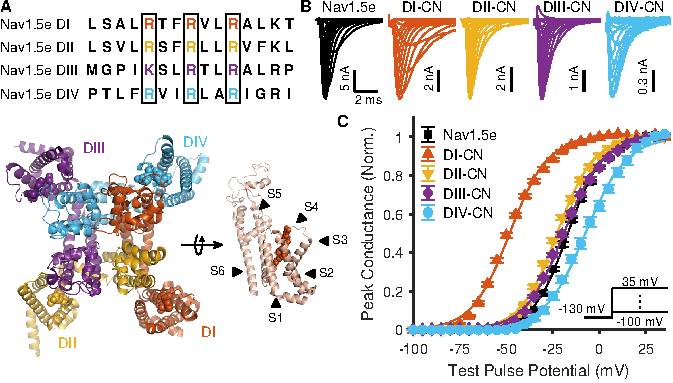
\includegraphics[width=115mm]{Figures/AppendixA/figure01.pdf}
\caption{\captiontitle{Impact of neutralizing voltage-sensing domains on channel activation.}
(A) Top: Sequence alignment of the S4 voltage-sensing helices across domains I-IV of mNav1.5e. Outlined in black are the gating charges that were neutralized to glutamine in the charge-neutralized (CN) mutants. Bottom: top-down view of the structure of Nav1.5 from (Jiang et al., 2020). To the right is a side view of domain I with the various transmembrane $\alpha$ helices annotated. Gating charges corresponding to those outlined in black boxes in the top of the panel are annotated as balls in the structure. 
(B) Representative traces of ionic currents corresponding to wild-type (WT) Nav1.5e (cell 20170418c2) and mutant channels (DI-CN, cell 20180307c1; DII-CN, cell 20180316c1; DIII-CN, cell 20180712c3; DIV-CN, cell 20190318c3) in response to depolarizing voltage steps ranging from -110 to 35 mV, following a holding potential of -130 mV (-100 mV for WT), recorded in HEK-293T cells. A scheme of this voltage step protocol is displayed in the inset of panel C. 
(C) Normalized peak conductance (GV) of wild-type and mutant channels. Inset: voltage step protocol used to assess channel activation. Solid lines are fitted Boltzmann curves. Parameter values are reported in \autoref{tab:AS1}. Similar data from adult Nav1.5 (mH1) is present in \autoref{fig:AS1}.}
\label{fig:A1}
\end{figure}

The voltage-dependent gating of Nav channels is distinct from the homotetrameric behaviour of voltage-gated potassium channels in that each Nav channel domain appears to have a differentiated role. For example, DI and DII movements are thought to play no role in inactivation, and function only to drive pore opening (Ahern et al., 2016; Armstrong and Hollingworth, 2018; Angsutararux et al., 2021). Several experiments have pointed to DIV playing a unique role in inactivation (Chen et al., 1996; Chanda and Bezanilla, 2002; Capes et al., 2013); however, other studies have pointed to a role for both DIII and DIV in inactivation (Cha et al., 1999; Hsu et al., 2017). To explain this, two gating models for Nav channels have been proposed, one in which both DIII and DIV movements are necessary for inactivation (Armstrong, 2006; Armstrong and Hollingworth, 2018), and another where DIV alone is sufficient for inactivation (Ahern et al., 2016; Capes et al., 2013). The idea that DIV alone is sufficient for inactivation derives primarily from studies on a single isoform, Nav1.4 (Chanda and Bezanilla, 2002; Goldschen-Ohm et al., 2013; Capes et al., 2013). It remains to be determined, therefore, the extent to which all Nav channels obey a common model of voltage-dependent gating. 

To test the hypothesis that all Nav channels follow the same gating scheme as Nav1.4, we characterized the role of each voltage sensor in the gating of Nav1.5e, a neonatal splice variant of the cardiac sodium channel. We mutated the first three gating charges in each S4 segment to glutamines, generating four charge-neutralized (CN) mutant channels: DI-CN, DII-CN, DIII-CN, DIV-CN. We also determined the steady-state behaviour of each voltage sensor using voltage-clamp fluorometry (VCF) experiments. Here, we report the results of these CN and VCF experiments and present detailed kinetic modelling which together reveal how each voltage sensor contributes to the macroscopic gating properties of Nav1.5 channels. Our results point to a critical role for closed-state inactivation in permitting voltage sensors to influence activation and inactivation properties. We show that Nav1.4, Nav1.5, and Nav1.6 all have different propensities for closed-state inactivation, and postulate that these differences produce isoform-dependent roles for the four voltage sensing domains.

\section{Methods}
\subsection{Molecular biology}
The mouse mH1 pcDNA3.1(+)-plasmid was obtained from Dr. T. Zimmer (Camacho et al., 2006). Exon 6a cDNA was amplified out of mouse brain homogenates, using the Access RT-PCR System (Promega), and then exchanged with exon 6b in mH1 using the Quikchange method of site-directed mutagenesis (SDM) (Braman et al., 1996), to generate the Nav1.5e plasmid.

Charge-neutralizing mutations of Nav1.5e were engineered using single-primer reaction in parallel (SPRINP) SDM (Edelheit et al., 2009). Primers (Integrated DNA Technologies) were designed containing both the amino acid exchanges of interest (\autoref{fig:A1}A) and a silent restriction site. Following the PCR reaction, unmutated templates were digested using 0.4-0.8 U/$\mu$L of DpnI (New England Biolabs). The resulting PCR mixture was transformed into house-grown competent DH5$\alpha$. Colonies were grown overnight on agar plates and picked for liquid culturing in 25 g/L Lysogeny Broth (Fisher Bioreagents). Plasmids were harvested using QIAprep Spin Miniprep Kits (Qiagen). Mutations were screened via restriction digest and gel electrophoresis, using the silent restriction sites initially designed into the SDM primers. Plasmid sequences were verified with Sanger sequencing done by the Innovation Centre of McGill University and Genome Quebec, using Sequencher 4.8 and CLC Sequence Viewer 8.0.

Nav1.5e DIV-CN constructs were modified further by conjugating the Nav sequence to an engineered GFP fluorophore called Mystik (Mys) via a P2A linker. The P2A allowed for the stoichiometric 1:1 translation of the Mystik and Nav genes, so that cells showcasing the strongest fluorescence were the most likely to express the Nav channel in higher abundance (Ahier and Jarriault, 2014). The allowed us to overcome the poor expression of Nav1.4 alone. Primers (Integrated DNA Technologies) with overhangs containing fragments of the Nav plasmid’s 5’ untranslated region or part of the P2A-Nav sequence were used to PCR amplify a double-stranded “megaprimer” containing (from 5’ to 3’): the 5’ UTR upstream of the Nav channel, the entire Mys gene, the P2A sequence, and the 5’ end of the Nav channel cDNA. This megaprimer was then isolated via gel electrophoresis, extracted into solution using MinElute Gel Extraction Kits (Qiagen), and inserted into the Nav channel plasmid by means of the Quikchange method of PCR discussed previously.

\subsection{Cell culture}
Human embryonic kidney cells mutated to over-express the SV40 large T-antigen (HEK-293T cells) were used as the expression system for electrophysiological recordings. HEK-293T cultures were maintained in minimal essential media containing Glutamax (MEM-glutamax; Gibco), supplemented with 10\% fetal bovine serum (FBS; Gibco), and kept at conditions of 37°C, 100\% humidity, and 5\% CO2 in a ThermoForma Series II Water-Jacketed CO2 Incubator (ThermoFisher). Main HEK-293T stocks were grown in T-25 Flasks (Corning) and twice a week passaged using Trypsin-EDTA solution (Gibco) into 35-mm Tissue-Culture Treated Culture Dishes (Corning) for transfection purposes. The calcium phosphate transfection protocol (Jordan et al., 1996) was used to transiently transfect HEK-293T cells at least 24 hours before recordings. Each 35-mm culture dish was loaded with 0.5 $\mu$g of the Nav channel plasmid, 0.2 $\mu$g of the transfection reporter Mys (unless already present, as in the Mys-P2A-Nav constructs). The cDNA mixture was dissolved in 560 mM of CaCl2 (unless otherwise indicated, all chemical reagents are from Sigma-Aldrich), and an equal volume of 2XBES solution (in mM: 50 BES, 280 NaCl, and 1.5 Na2HPO4) was added to induce precipitate formation. After roughly one minute, the DNA-calcium phosphate precipitates were added to a single culture dish. The dish was then returned to the incubator where cells had time to be transfected, typically over 6 to 9 hours. The reaction was quenched 6 to 9 hours later by rinsing with phosphate-buffered saline (PBS, in mM: 137 NaCl, 2.7 KCl, 10.1 Na2HPO4, and 2 NaH2PO4) containing 1 mM EDTA and rinsed with PBS containing 1 mM MgCl2 and 1 mM CaCl2. Transfected HEK-293T cells were left to recover overnight.

\subsection{Electrophysiology}
At least two hours before the start of recordings, transfected cells were dissociated from their cultures using Accutase and then re-plated at a lower density. This step increased the yield of isolated cells, minimizing gap junctions that form between adjacent HEK-293T cells and optimizing the quality of the voltage-clamp conditions. Culture media was replaced with external solution containing (in mM): 155 NaCl, 4 KCl, 5 HEPES, 1 MgCl2, and 1.8 CaCl2, with pH adjusted to 7.3-7.4 using NaOH. Cells were patched with microelectrodes containing an internal solution that was optimized for voltage-clamp conditions, made up of (in mM): 115 CsCl, 5 HEPES, 5 Cs4-BAPTA, 1 MgCl2, 0.5 CaCl2, 10 Na2ATP, with pH adjusted to 7.3-7.4 using CsOH and sucrose added to keep the osmolality matching that of the external solution, between 295-300 mOsm. Borosilicate glass capillaries --- with an inner diameter of 1.15 mm, an outer diameter of 1.65 mm, a length of 100 mm, and a 0.1 mm filament (King Precision Glass, Inc) --- were pulled using a PP-830 vertical puller (Narishige), yielding microelectrodes with a pipette resistance of 1 to 5 MΩ. Microelectrode tips were then dipped into Bees-Wax Pure Natural (Integra Miltex) and subsequently fire-polished with an MF-900 Micro Forge (Narishige), to reduce noise and improve membrane seals. Dissociated cells were viewed using an Eclipse Ti-U Inverted Microscope (Nikon). Transfected cells were identified by their green fluorescence, excited by a DC4104 4-Channel LED Driver (Thorlabs). Positive pressure was applied orally to electrodes before being lowered to the bottom of the recording chamber using an MP-285 micromanipulator (Sutter Instrument). Once the electrode tip was positioned just above the surface of the cell, the release of the positive pressure was sufficient to form a glass-membrane seal of at least 1 GΩ. Pulses of negative pressure were then delivered to improve the strength of the seal and eventually break through, giving access to the whole-cell patch-clamp configuration. All recordings were done at room temperature.

Voltage commands were delivered through an AxoPatch 200B Amplifier (Axon Instruments). Capacitive transients from the pipette and from the cell were cancelled, cell capacitance and series resistance were monitored to avoid changes exceeding 30\% over the course of the recording, and series resistance was compensated to the amplifier’s maximum (98\% on the machine, but in practice probably closer to 80\%). Currents were acquired at 100 kHz, low-pass Bessel filtered at 5 kHz using a Model 900 Tunable Active Filter (Frequency Devices), and telegraphed via an Axon Digidata 1550 (Molecular Devices). All data was collected and saved digitally using pClamp 10.7 software (Axon Instruments).

\subsection{Voltage-clamp protocols}
When cells were not being recorded, either between protocols or between sweeps within a protocol, they were clamped at a holding potential of -60 mV. To assess channel activation, cells were stepped down to the baseline potential for 300 ms, depolarized to a series of potentials between -110 and +70 mV in increments of 5 mV for 100 ms, then returned to the baseline potential for another 300 ms. This baseline potential was either -100 mV for Nav1.5e, or -130 mV in the case of the charge-neutralized mutants, to counter the latter’s increased propensity for channel inactivation. To assess steady-state inactivation, cells were stepped down to the baseline potential for 300 ms, given a pre-pulse that varied between -160 mV and -5 mV in increments of 5 mV for 100 ms, pulsed directly to the test pulse potential of -10 mV for 50 ms, then returned to -100 mV for an additional 300 ms. Leak subtraction was performed on the raw data in a custom Igor Pro (Wavemetrics) program post-hoc. 

\subsection{Voltage-clamp fluorometry}
All experiments conducted on Xenopus laevis were done with the approval of and according to the guidelines established by the Animal Care Committee of the National Institutes of Natural Sciences, an umbrella institution of the National Institute for Physiological Sciences. We obtained the Nav1.5 VCF constructs used by Varga et al. (Varga et al., 2015) from J.R. Silva (Washington University in St. Louis) and used site-directed mutagenesis, as described previously, to convert them to their respective Nav1.5e variants (with the exception of position 215, which was not mutated to leucine because it was used as a labelling cysteine). The four Nav genes, inserted on pMax vectors, could be linearized using Pacl (TOYOBO) and used as a template to generate cRNA using the mMESSAGE T7 RNA transcription kit (Thermo Fisher Scientific). 

The oocytes of Xenopus laevis were surgically harvested from anaesthetized animals as described previously (Kume et al., 2018). Oocytes were separated ad defolliculated using 2 mg/ml collagenase treatment for 6.5 hours. Then oocytes were incubated overnight at 17\textdegree C in Ringer’s solution containing (in mM): 88 NaCl, 1 KCl, 2.4 NaHCO3, 0.3 Ca(NO3)2, 0.41 CaCl2, 0.82 MgSO4, and 15 HEPES, with pH adjusted to 7.4 with NaOH and use of 0.1\% penicillin-streptomycin. The remaining follicular layers were manually peeled. 25 ng of Nav channel cRNA was injected into the vegetal pole of oocytes using Nanoject II (Drummond). Treated oocytes were then returned to their 17\textdegree C incubator and left for 1 to 3 days to express protein.

Oocytes were labelled for 20 minutes using 10 $\mu$M of methanethiosulfonate-carboxy\-tetra\-methyl\-rhodamine (MTS-TAMRA) dye on ice. Dye conjugation was done in depolarizing solution (containing, in mM, 110 KCl, 1.5 MgCl2, 0.8 CaCl2, 0.2 EDTA and 10 HEPES, pH adjusted to 7.1 with KOH) in an effort to expose and label S4 helices. Excess dye was removed by rinsing five times with fresh ND-96 solution (96 mM NaCl, 2 mM KCl, 1.8 mM CaCl2, 1 mM MgCl2, 5 mM HEPES, with pH adjusted to 7.4 wit NaOH). Oocytes in solution were kept on ice until use. Eventually, oocytes were transferred to the recording chamber filled with ND-96 solution, at room temperature, oriented in such a way that fluorescent recordings were done on the animal pole. Voltage clamp for macroscopic current recording was performed by using an amplifier (OC-725C, Warner Instruments). Borosilicate glass capillaries (World Precision Instruments) were used with a resistance of 0.1–0.3 MΩ when filled with 3 M KOAc and 10 mM KCl. The fluorescent recordings were performed with the fluorescence microscope (Olympus BX51WI) equipped with a water immersion objective lens (Olympus XLUMPLAN FL 20x/1.00). The light source was emitted by a xenon arc lamp (L2194-01, Hamamatsu Photonics) and passed through a band-pass excitation filter (520-550 nm). The intensity of the excitation light was decreased to prevent the fluorophore from bleaching by ND filters (Olympus U-25ND6 and U-25ND25). Emitted light was passed through a band-pass emission filter (580IF). The emission signals were detected by a photomultiplier (Hamamatsu Photonics H10722-110). The baseline signal was adjusted to 2 V. The detected current and fluorescent signal were acquired by a Digidata 1332 (Axon Instruments) and Clampex 10.3 software (Molecular Devices) at 100 kHz.

Oocytes were held at a baseline of -60 mV between sweeps and protocols. Once we could detect a visible change in fluorescence upon depolarization of the oocyte from -120 mV to +60 mV, we could run the following activation protocol. The oocyte was stepped down to -120 mV for about 300 ms, then hyperpolarized/depolarized to a series of potentials between -180 mV and +60 mV in increments of 10 mV for 100 ms, then stepped back to -120 mV for about 300 ms before returning to baseline. The protocol was run and averaged 10 times to improve the signal-to-noise ratio in the fluorescent output. Voltage-clamp fluorometry data was analyzed automatically using custom-made Igor Pro scripts.

\subsection{Data analysis and statistics}
For activation, ENa was determined by fitting the linear part of the current-voltage curve to a line and extrapolating its x-intercept. Conductance was calculated as $I/(V-ENa)$, then fit with a Boltzmann function
\begin{equation}
G\left(V\right)=\frac{G_{max}}{1+e^{-\ \frac{V-V_{1/2}}{k}}},
\end{equation}
where Gmax is the maximum conductance, V\textsubscript{1/2} is the half-activation potential, and k is the slope factor of voltage sensitivity. For steady-state inactivation, peak currents following the test pulse were plotted against the corresponding pre-pulse potential; a Boltzmann function was then fit to this I-V curve. To calculate time to peak, the maximum current occurring at least 0.5 ms following the voltage step was identified (to avoid identifying capacitive transients at low voltages). The latency from the moment of voltage step to this peak was calculated. Recovery rates were determined by fitting each recovery curve to the equation, $f\left(t\right)=A\exp{(\alpha_1t)}+\left(1-A\right)\exp{\left(\alpha_2t\right)}$ and was defined as $\alpha_w=A\alpha_1+\left(1-A\right)\alpha_2$.

To experimentally quantify the fraction of inactivation occurring from closed states (i.e. closed-state inactivation), we adapted the method proposed by Armstrong (Armstrong, 2006). Briefly, open-state inactivation was estimated during a conditioning voltage step (80 ms long, ranging from -160 to -5 mV), and then compared to the fraction of available channels during a subsequent test pulse (-10 mV), thereby estimating the fraction of steady-state inactivation occurring through open states. Closed-state inactivation was then defined as the complementary fraction. Specifically, open-state inactivation (OSI) was estimated by the equation
\begin{equation}
OSI\left(V\right)\propto\sum_{t=0}^{\tau}{g\left(t;V\right)\ \Delta t},
\end{equation}
where $g(t;V)$ is the experimentally observed channel conductance at time t for voltage step V. In the original method (Armstrong, 2006), OSI was scaled by assuming 100\% of steady-state inactivation occurs from open states at 0 mV. However, our data displayed significantly more closed-state inactivation than was observed by Armstrong (Armstrong, 2006) and consequently OSI did not necessarily attain a maximum within the tested voltage range. We therefore modified this method by fitting a Boltzmann function, $f\left(V\right)=\alpha\left(1+e^{-\left(V-V_{1/2}\right)/k}\right)^{-1}$, to the unscaled OSI versus voltage curve to obtain a scaling factor, i.e. $\alpha$. This allowed open-state inactivation to attain its maximum outside of the observed voltage range.

For statistical analysis, Tukey’s method was used following a one-way ANOVA, with a significance level of $p<0.01$. All data is reported as mean ± SEM. 

\subsection{Modelling}
For simulations of Nav channel conductance, two gating schemes were used in the study. The first, which we refer to as Gating Scheme I is precisely the kinetic model of Nav1.4 developed by Capes et al. (Capes et al., 2013) (\autoref{fig:A3}A). The second, which we refer to as Gating Scheme II, is described in the final section of the Results (\autoref{fig:A10}). Both schemes were fit to Nav1.5e data with a custom-made evolutionary fitting algorithm programed in MATLAB 2017b (The MathWorks, Inc.). Microscopic reversibility was enforced. Goodness of fit was assessed on z-scores calculated with respect to our experimental observations of the integral, peak amplitude, and time to peak of the activation and inactivation currents, as well as the recovery from inactivation, steady-state inactivation, and activation IV curves. The resulting parameter values for Scheme I are reported in \autoref{tab:AS2} and those for Scheme II are reported in \autoref{tab:AS4}.
When performing the two-parameter sensitive analysis in \autoref{fig:A3}, the first three rightward transitions were accelerated by altering the rate $\alpha$. Since the final rightward transition is governed by different rates for each row, whenever the rate $\gamma$ was increased or decreased, the rates $\gamma_4$ and $\gamma_i$ were also changed by the same amount to uniformly alter the final rightward transition. Anywhere it is stated that $\gamma$ is altered, it is implied that the rates $\gamma_4$ and $\gamma_i$ were also altered commensurately.
All simulations were reported with custom routines written in MATLAB code. As all applied voltage protocols were step functions, solutions to the model were computed using the exponential of the matrix of transition rates. Stochastic simulations were run using the Gillespie algorithm. 	

\subsection{Data and materials availability}
All the code and data used in the generation of figures is publicly available at \url{https://github.com/niklasbrake/Nav2022}. Raw data is available upon request from the authors.

\subsection{Online Supplemental Material}
Supplemental \hyperref[fig:AS1]{Figures} \ref{fig:AS1} and \ref{fig:AS3} parallel  \hyperref[fig:A1]{Figures} \ref{fig:A1} and \ref{fig:A5} and show data for charge neutralized adult Nav1.5 (mH1) channels.  \hyperref[fig:AS2]{Figure} \ref{fig:AS2} demonstrates the relationship between first open latency and time to peak current for Gating Scheme I. \hyperref[fig:AS4]{Figure} \ref{fig:AS4} shows the fit of Gating Scheme II to Nav1.5e data. \autoref{tab:AS1} presents the summary data for activation, inactivation, and recovery of Nav1.5e and the four CN mutants. \autoref{tab:AS2} presents the parameters used to fit Gating Scheme I to Nav1.5e data. \autoref{tab:AS3} presents summary VCF data. \autoref{tab:AS4} presents the parameters used to fit Gating Scheme II to Nav1.5e data. \autoref{tab:AS5} report the parameter changes to refit Gating Scheme II to CN mutant data or to adult Nav1.5 data.

\section{Results}
\subsection{Voltage Sensor Charge Neutralization Identifies the Dominant Role of DI in Channel Activation}
Wildtype Nav1.5e as well as the four CN mutants were characterized in HEK-293T cells transiently transfected with cDNA. To assess channel activation, macroscopic Na+ currents were recorded while applying depolarizing voltage steps in increments of +5 mV (range, -110 and +55 mV), each from a holding potential of -130 mV (-100 mV for wildtype channels) (\autoref{fig:A1}B). The voltage-dependence of channel activation for wildtype and mutant channels was then determined by fitting the peak conductance (G/V) with a Boltzmann function (\autoref{fig:A1}C). 

The activation profiles of DI, DII, and DIV-CN mutant Nav1.5e channels were significantly different from WT, with DI charge neutralization producing the greatest impact (\autoref{fig:A1}C). Fits of peak G/V relationships estimated the voltage for half-maximal activation (V\textsubscript{1/2}) to be -16.8 ± 0.45 mV (n = 51) for wildtype channels compared to -48.1 ± 0.55 mV (n = 24) for DI-CN (\autoref{fig:A1}C, \autoref{tab:AS1}), representing a 30 mV hyperpolarizing shift in channel activation (Q = 57.2; d.f. = 131; k = 5; $p < 10^{-12}$, Tukey’s range test, significance threshold: $p < 0.0$1). In contrast, charge neutralization of DII and DIII had a more modest effect on channel activation with V\textsubscript{1/2} values of -22.6 ± 0.54 mV (n = 26) and -19.0 ± 0.58 mV (n = 23), respectively (\autoref{fig:A1}C), corresponding to hyperpolarizing shifts in activation of about 6 mV (Q = 10.8, $p < 10^{-9}$) and 2 mV (Q = 3.91, $p = 0.05$). Finally, charge neutralization of DIV had the opposite effect on channel activation, shifting the V\textsubscript{1/2} value to -7.4 ± 1.26 mV (n = 14) (\autoref{fig:A1}C), representing a +10 mV depolarizing shift in channel activation compared to wildtype Nav1.5e (Q = 11.9, $p < 10^{-9}$). Similar relative shifts in channel activation were observed when DI through to DIV voltage sensors were charge neutralized in the adult form of Nav1.5 (i.e. mH1), demonstrating that our observations are not specific to the neonatal form of Nav1.5 (\autoref{fig:AS1}). Our observations of Nav1.5 are comparable with previous findings on skeletal muscle Nav1.4 channels, with the exception of DIV-CN which did not depolarize activation in Nav1.4 (Capes et al., 2013).

\subsection{DI Movement Is the Rate-Limiting Step for Pore Opening}
To understand the varied effects of VSD neutralization, we adapted a past Markov gating model of Nav1.4 (Capes et al., 2013) (\autoref{fig:A2}A). This model (Gating Scheme I) encapsulates the view that DI-III movements are necessary for pore opening and DIV movement is sufficient and rate-limiting for inactivation (Ahern et al., 2016). We re-fit the model parameters, allowing the model to successfully capture several functional properties of Nav1.5e wildtype channels, including its activation, inactivation, and recovery from inactivation behaviours (\autoref{fig:A2}, \autoref{tab:AS2}). 

\begin{figure}[t]
\begin{minipage}[c]{85mm}
    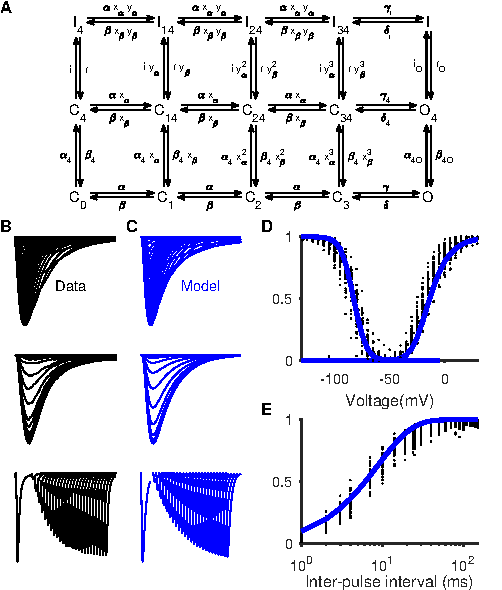
\includegraphics[width=\textwidth]{Figures/AppendixA/figure02.pdf}
\end{minipage}\hfill
\begin{minipage}[c]{80mm}
    \caption{\captiontitle{Gating Scheme I fitted to Nav1.5e data.}
    (A) A re-parameterized kinetic model of Nav gating, adopted from Capes et al. (2013) -- referred to here as Gating Scheme I. Horizontal transitions from left to right represent the nonspecific movement of DI-III, followed by pore opening. Vertical transitions from bottom to top represent the movement of DIV followed by the movement of the inactivation gate.
    (B) From top to bottom, averaged currents recorded from WT Nav1.5e channels during the activation protocol (as in \autoref{fig:A1}), inactivation protocol (currents elicited by a text pulse to -10 mV, following a conditioning pulse ranging from -160 to -5 mV), and recovery from inactivation protocol (currents elicited by a test pulse of -10 mV, following a holding potential of -10 mV and a hyperpolarizing inter-pulse of -100 mV lasting between 1-150 ms). 
    (C) Model outputs of Gating Scheme I parameterized with the values present in \autoref{tab:AS2}.
    (D) Steady-state inactivation (left) and GV (right) curves compute from data (black) and model (blue).
    (E) Fraction of recovered current as a function of inter-pulse interval for the WT channel (black) and model (blue).}
    \label{fig:A2}
\end{minipage}
\end{figure}


It has been proposed that DI-CN hyperpolarizes G/V relationship because DI movement is rate-limiting for pore opening (Capes et al., 2013). Based on this rationale, DIV-CN could depolarize activation by slowing the rate of pore opening. We explored this possibility using the kinetic gating model, where the rates that determine the transitions from the resting state to the open state are $\alpha$ and $\gamma$ (see Methods). To investigate how the voltage-dependence of the G/V relationship depends on these rates, we performed a sensitivity analysis with respect to both rates (\autoref{fig:A3}A). Notably, when $\alpha$ and $\gamma$ were varied slightly from the fitted parameters, the V\textsubscript{1/2} of activation was only sensitive to the rate $\gamma$. However, when $\gamma$ was much faster, the V\textsubscript{1/2} did not change and was only sensitive to the rate $\alpha$ (\autoref{fig:A3}A). This observation precisely shows that altering a transition to pore opening only impacts the V\textsubscript{1/2} of activation if the transition was slow compared to the other transitions, i.e. rate limiting. To show this directly, we simulated latencies to first pore opening by running stochastic simulations of the gating model. We found that shifts in G/V relationship were associated with similar shifts in median first latency times (\autoref{fig:A3}A). In fact, these results indicated that changes to the activation pathway depolarized the G/V relationship only if they also slowed the latency to first channel opening (\autoref{fig:A3}A). The model predicts, therefore, that if DI movement is rate-limiting for pore opening, then DI-CN should have faster latencies to pore opening. Importantly, if DIV-CN promotes a depolarization shift in the G/V relationship by affecting the activation pathway, then it must slow the latency to pore opening (\autoref{fig:A3}A). For macroscopic current recordings, the model predicts that if DI-CN accelerates pore opening, then DI-CN mutant channels should display faster current rise times (\autoref{fig:A3}B-D; \autoref{fig:AS2}). Conversely, if DIV-CN channels slow activation, we would expect them to display slower current rise times (\autoref{fig:A3}D; \autoref{fig:AS2}).

\begin{figure}[t]
\centering
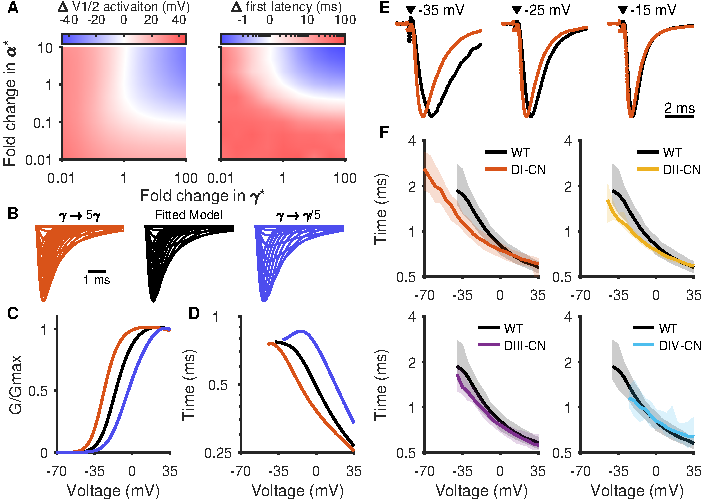
\includegraphics[width=120mm]{Figures/AppendixA/figure03.pdf}
\caption{\captiontitle{A model of Nav gating predicts changes in current rise time.}
(A) Left: Sensitivity analysis for V\textsubscript{1/2} of activation with respect to parameters $\alpha$ and $\gamma$ (see Methods). The point (1,1) indicates the baseline parameters fitted to the data (\autoref{fig:A2}). Bluer hues indicate a more hyperpolarized activation curve while redder hues indicate depolarized activation curves. Right: the average time to first pore opening, i.e. first latency, was computed for various values $\alpha$ and $\gamma$ following a voltage step from -130 mV to -30 mV. Bluer and redder hues indicate fast and slower latencies, respectively, with respect to baseline parameters.
(B) Middle: Representative traces of the WT Nav1.5 model response to the activation protocol. Right: $\gamma$* has been decreased 10-fold to simulate a slower activation rate. Left: $\gamma$* has been increased 5-fold to simulate a faster activation rate.
(C) GV plots calculated from the traces of corresponding colour in panel B. 
(D) Time to peak current calculated from the traces of corresponding colour in panel B. 
(E) Representative traces showing the current (normalized to peak amplitude) elicited by the indicated voltage steps for WT (black; cell 20170428c1) and DI-CN mutant channels (red; cell 20180307c1). 
(F) Time to peak current induced by voltage pulses ranging between -75 and 30 mV, starting from a holding potential of -130 mV, for Nav1.5e (black) and the four CN mutants. Line represents median while shading is 5-95\% quantile interval. Time to peak was not calculated at voltages that did not elicit a current.
}
\label{fig:A3}
\end{figure}

To test these model predictions, we measured the latency to peak current of each mutant Nav channel (\autoref{fig:A3}E, F). As anticipated, DI-CN channels displayed faster rise-times at hyperpolarized membrane potentials (\autoref{fig:A3}F), suggesting that DI movement is rate-limiting for pore opening. The rise-times of DII-CN and DIII-CN mutant channels were consistent with their more modest impacts on the V\textsubscript{1/2} of channel activation (Figs. 1C \& 3F). DIV-CN mutants did not display different response rise-times relative to WT channels (\autoref{fig:A3}F). This observation suggests that neutralizing DIV does not change the rate of pore opening, consistent with the idea that DIV is not directly involved in the activation process (Ahern et al., 2016). We therefore concluded that DIV-CN must shift the G/V relationship through a separate mechanism.

\subsection{Neutralizing DIV depolarizes activation by increasing inactivation from closed states}
The foregoing results suggest that DIV-CN affects the G/V relationship through alterations in the inactivation pathways. To investigate this further, we determined how Gating Scheme I would behave upon increasing the propensity of DIV to transition from its resting to its active state. We accomplished by increasing the DIV forward rates $\alpha_4$ and $\alpha_{4O}$ by 20-fold and by decreasing the DIV backward rates $\beta_4$ and $\beta_{4O}$ by 20-fold (\autoref{fig:A4}A). Surprisingly, biasing DIV led to a depolarizing shift in the G/V relationship (\autoref{fig:A4}B, D), consistent with our experimental observations from Nav1.5e DIV-CN mutants (\autoref{fig:A1}C). The reason we obtain such behaviour is because the voltage-dependence of activation is determined by the voltage when pore opening occurs faster than inactivation (\autoref{fig:A4}C), whereupon channel inactivation shifts from closed-state inactivation (CSI) to open-state inactivation. When DIV-CN is simulated, inactivation is faster (\autoref{fig:A4}E), shifting the balance towards CSI and thus requiring more depolarized voltages for pore opening to outcompete inactivation. These modelling results thus demonstrate that the effect of neutralizing DIV on the G/V relationship is consistent with DIV movement being rate-limiting for inactivation (Capes et al., 2013).

\begin{figure}[t]
\begin{minipage}[c]{85mm}
    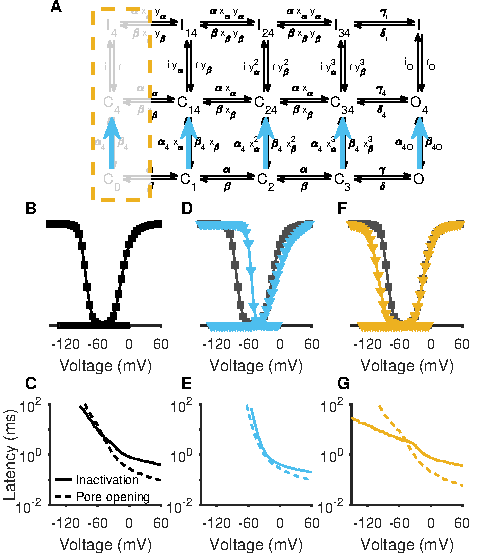
\includegraphics[width=\textwidth]{Figures/AppendixA/figure04.pdf}
\end{minipage}\hfill
\begin{minipage}[c]{80mm}
    \caption{\captiontitle{GV consequences of DIV-CN is consistent with removing rate-limiting step for inactivation.}
    (A) A schematic depicting how CN was simulated in the gating model. The leftmost column of states was removed to simulate the charge neutralization of a non-specific domain whose movement is necessary for pore opening (yellow). We refer to this model as the DII-CN model. The rates $\alpha_4$ and $\alpha_{4O}$ were increased 20-fold and $\beta_4$ and $\beta_{4O}$ were decreased 20-fold to approximate the removal of the bottom row, thereby simulating DIV-CN (blue).
    (B) The GV and SSI curves produced by the model prior to any manipulations (identical to \autoref{fig:A2})
    (C) The median latency to first DIV movement (solid line) and first pore opening (dashed line) were determined at a range of voltages from stochastic simulations of the gating model. This panel shows that the GV curve in panel B is non-zero at voltages where pore opening occurs faster on average that channel inactivation.
    (D) The GV and SSI curves produced by the model following simulated DIV-CN (blue) overlayed with the original curves from panel B (black). SSI is hyperpolarized and GV is depolarized in the DIV-CN model.
    (E) Same as panel C, but for the DIV-CN model. The rate of inactivation is faster, while the rate of pore opening is relatively unchanged. 
    (F-G) Same as panels D-E, but for the DII-CN model. The SSI curve is hyperpolarized and the GV curve is unchanged in the DII-CN model. The rate of inactivation is faster at hyperpolarized potentials.}
    \label{fig:A4}
\end{minipage}
\end{figure}

We next asked whether the model could also capture the (lack of) effect of DII- and DIII-CN on the G/V relationship. Since the first three activation transitions in Gating Scheme I all use the same rates, each transition could not be independently altered. We therefore simply removed the leftmost column of the model, consisting of the states C0, C4, and I4 (\autoref{fig:A4}A). This is equivalent to assuming that the first step in the activation process is already complete; that is, the relevant domain has been biased towards its “active” conformation. Although this manipulation did not affect channel activation, it unexpectedly produced a leftward shift in the SSI curve (\autoref{fig:A4}F). This leftward shift occurred because of positive cooperativity between channel activation and inactivation ($x_\alpha/x_\beta>1$, $y_\alpha/y_\beta>1$; see \autoref{tab:AS2}): removing the first column of states accelerated the rate of CSI, thereby increasing the total amount of SSI (\autoref{fig:A4}F, G). We tested this prediction in the following sections.
	
\subsection{All Voltage Sensors Contribute to Steady-State Inactivation of Nav1.5e Channels}
Steady-state inactivation (SSI) of wildtype and mutant Nav1.5e channels was determined by applying a 100 ms-long conditioning pulse (range, -160 to -5 mV) followed by a test pulse of -10 mV to elicit Na+ currents (\autoref{fig:A5}A, B). SSI plots were then constructed by fitting the peak response at each test potential with a Boltzmann function (\autoref{fig:A5}C). The largest impact on SSI occurred from neutralizing DIV, shifting the V\textsubscript{1/2} from -82.0 ± 0.52 mV in wildtype channels to -131.1 ± 2.55 mV (n = 13) in DIV-CN mutants (Q = 27.6, d.f. = 126, k = 5, $p < 10^{-15}$; Tukey’s range test). The slope factor for the inactivation curve was significantly flatter for DIV-CN mutants (k = -13.7 ± 1.46, n = 13) than for wildtype Nav1.5e channels (k = -7.2 ± 0.14, n = 49) (Q = 18.1, d.f. = 126, k = 5, $p < 10^{-5}$; Tukey’s range test), indicating a lower sensitivity to membrane potential. Charge neutralization of DIII affected SSI in a manner similar to neutralizing DIV, hyperpolarizing the V\textsubscript{1/2} of inactivation by 40 mV to -120.0 ± 1.09 mV (n = 23) (Q = 26.0, $p < 10^{-15}$) and flattening the SSI slope factor to -14.4 ± 0.15 (n = 23) (Q = 14.2, $p < 10^{-12}$). Although measurements of SSI for DI and DII-CN mutants differed from wildtype Nav1.5e, the shift was less than for DIII and DIV-CN mutants. The V\textsubscript{1/2} of inactivation was estimated to be -100.9 ± 0.54 mV (n = 23) and -96.5 ± 0.82 mV (n = 25) for DI and DII-CN mutants, respectively (\autoref{fig:A5}C), corresponding approximately to 20 mV (Q = 12.9, $p < 10^{-9}$) and 15 mV (Q = 10.3, $p < 10^{-9}$) hyperpolarizing shifts. Similar relative shifts in SSI were also observed from charge-neutralized adult Nav1.5 channel mutants (\autoref{fig:AS3}), again demonstrating that our observations are not specific to the neonatal form of Nav1.5.

\begin{figure}[t]
\begin{minipage}[c]{85mm}
    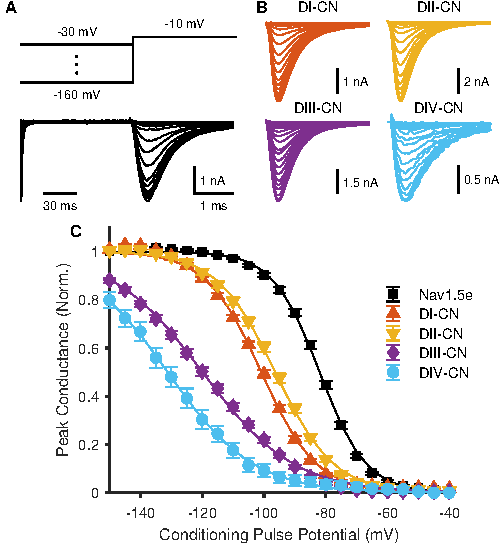
\includegraphics[width=\textwidth]{Figures/AppendixA/figure05.pdf}
\end{minipage}\hfill
\begin{minipage}[c]{80mm}
    \caption{\captiontitle{GV consequences of DIV-CN is consistent with removing rate-limiting step for inactivation.}
    (A) A schematic depicting how CN was simulated in the gating model. The leftmost column of states was removed to simulate the charge neutralization of a non-specific domain whose movement is necessary for pore opening (yellow). We refer to this model as the DII-CN model. The rates $\alpha_4$ and $\alpha_{4O}$ were increased 20-fold and $\beta_4$ and $\beta_{4O}$ were decreased 20-fold to approximate the removal of the bottom row, thereby simulating DIV-CN (blue).
    (B) The GV and SSI curves produced by the model prior to any manipulations (identical to \autoref{fig:A2})
    (C) The median latency to first DIV movement (solid line) and first pore opening (dashed line) were determined at a range of voltages from stochastic simulations of the gating model. This panel shows that the GV curve in panel B is non-zero at voltages where pore opening occurs faster on average that channel inactivation.
    (D) The GV and SSI curves produced by the model following simulated DIV-CN (blue) overlayed with the original curves from panel B (black). SSI is hyperpolarized and GV is depolarized in the DIV-CN model.
    (E) Same as panel C, but for the DIV-CN model. The rate of inactivation is faster, while the rate of pore opening is relatively unchanged. 
    (F-G) Same as panels D-E, but for the DII-CN model. The SSI curve is hyperpolarized and the GV curve is unchanged in the DII-CN model. The rate of inactivation is faster at hyperpolarized potentials.}
    \label{fig:A5}
\end{minipage}
\end{figure}

\subsection{Nav Channels Exhibit Different Degrees of Closed-State Inactivation}
Our data shows that neutralizing Nav1.5 voltage sensors affects channel activation and inactivation differently than reported for Nav1.4 channels (Capes et al., 2013). Specifically, DIV-CN depolarizes activation in Nav1.5, but not in Nav1.4, and DI-III hyperpolarizes SSI in Nav1.5, but not in Nav1.4. The differences in DI-, DII-, and DIV-CN can nevertheless be explained by a single gating scheme. Because CSI is central to the proposed mechanisms (\autoref{fig:A4}), we hypothesized that Nav1.4 and Nav1.5 may display different degrees of CSI. To explore variation in inactivation among Nav channels, we collected data from three different Nav channels: namely, skeletal muscle Nav1.4 channels, cardiac Nav1.5 channels, and neuronal Nav1.6 channels. 

To do this, we measured the fraction of inactivation occurring from open states (open-state inactivation, i.e. OSI) in each Nav isoform during 80 ms voltage steps ranging from -160 mV to -5 mV (\autoref{fig:A6}A, B) (see Methods). We then fit Boltzmann functions to the resulting OSI-voltage curves in order to quantify its voltage dependence. In Nav1.5e, the V\textsubscript{1/2} of OSI was -31.2 ± 0.4 mV (n=48), which was significantly more hyperpolarized than Nav1.4 (-21.4 ± 0.5 mV, n=21) ($p < 10^{-9}$; Tukey’s range test, k=3, d.f.=88) and Nav1.6 (-22.0 ± 0.2 mV, n=22) ($p < 10^{-9}$). The OSI of Nav1.4 and Nav1.6 did not display distinct voltage dependences ($p=0.67$). Overall, OSI followed a similar trend to SSI: SSI was also more hyperpolarized in Nav1.5e (\autoref{fig:A5}C) compared to Nav1.4 (-65.0 ± 0.4 mV, n = 21; $p < 10^{-9}$) and Nav1.6 (-55.7 ± 0.6 mV, n = 26; $p < 10^{-9}$) (\autoref{fig:A6}C). However, unlike OSI, SSI had a significantly different voltage dependence between Nav1.4 and Nav1.6, with Nav1.6 displaying a more depolarized SSI curve ($p<10^{-9}$) (\autoref{fig:A6}C). This latter finding demonstrates that SSI and OSI can vary independently of each other among different Nav channel isoforms. 

\begin{figure}[t]
% \begin{minipage}[c]{115mm}
    \centering
    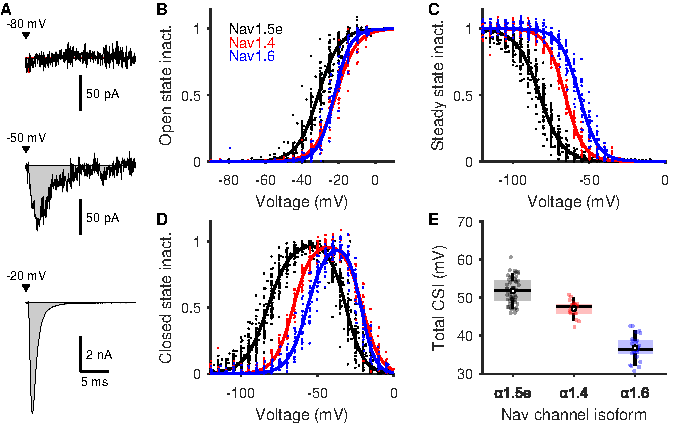
\includegraphics[width=115mm]{Figures/AppendixA/figure06.pdf}
% \end{minipage}\hfill
% \begin{minipage}[c]{60mm}
    \caption{\captiontitle{Closed-state inactivation is variable among Nav isoforms.}
    (A) Representative Nav1.5e currents in response to voltage steps from -130 mV to -80 (top), -50 (middle), and -20 mV (bottom). The amount of open state inactivation (OSI) at each voltage was computed based on the integral of these transient currents (grey shading). See Methods for details.
    (B) Amount of OSI at voltages ranging from -90 to -5 mV for three Nav isoforms: Nav1.5e (black), Nav1.4 (red), and Nav1.6 (blue). Dots are values from individual recordings and solid lines are fitted Boltzmann curves. Boltzmann parameters are reported in the text.
    (C) SSI curves of the three Nav channel isoforms. Boltzmann parameters are reported in the text.
    (D) Closed-state inactivation (CSI) was computed as the difference between SSI and OSI. Solid lines are the difference of two Boltzmann functions fitted to the data. 
    (E) Total CSI was defined as the integral of the CSI curves reported in panel D. Coloured dots represent individual cells. The white dots report the mean values for each isoform, while the black lines and shading represent box plots of the data. The Nav channel isoforms display distinct levels of total CSI.}
\label{fig:A6}
% \end{minipage}
\end{figure}

We next investigated CSI in each Nav channel isoform. Because all steady-state inactivation not occurring from an open state must have occurred directly from a closed state, we computed CSI as the difference between OSI and SSI (Armstrong, 2006). For Nav1.5e, CSI peaked at 100\% of all steady-state inactivation and remained high for a large range of voltages (\autoref{fig:A6}D). On the other hand, Nav1.4 displayed a smaller but still substantial level of CSI (\autoref{fig:A6}D) with Nav1.6 displaying the least amount. To quantitatively compare CSI between isoforms, we fit the CSI curves with the difference of two Boltzmann curves; the integral of this function was defined to be the total amount of CSI (\autoref{fig:A6}D). This analysis confirmed that the isoforms exhibited three distinct levels of CSI, with Nav1.5e displaying the most CSI, followed by Nav1.4 and finally Nav1.6 (\autoref{fig:A6}E). Overall, these data demonstrate that CSI of the Nav channel isoforms is different.

\subsection{Degree of closed state inactivation determines consequences of voltage sensor neutralization}
Given these findings, we aimed to determine whether lower CSI indeed leads to a more Nav1.4-like behaviour following domain neutralization. To test this, we modified the Nav1.5 parameterization of Gating Scheme I to decrease the amount of CSI. We forced DIV to move exclusively following pore opening by decreasing the likelihood of DIV movement prior to pore opening ($\alpha_4$ decreased by 20-fold and $\beta_4$ increased by 20-fold), and increasing the likelihood of DIV movement following pore opening (4 increased by 20-fold and $\beta_{4O}$ decreased by 20-fold) (\autoref{fig:A7}A). As expected, this parameter manipulation significantly reduced the amount of CSI compared to the original Nav1.5e model (\autoref{fig:A7}B). To understand how the sequential order of domain activation was altered, we measured the median latency to DIV movement and compared this against latency to DI-III movement in stochastic simulations of the two models; these simulations confirmed that the low CSI model followed a strict DIV-last domain movement order, unlike the Nav1.5e model where DIV consistently moved prior to DI-III at all voltages less than -50 mV (\autoref{fig:A7}C).
Simulating DII-CN with this “low CSI” parameterization did not appreciably alter gating (\autoref{fig:A7}D), consistent with experimental observations of Nav1.4 (Capes et al., 2013). Similarly, simulating DIV-CN, as previously done (\autoref{fig:A4}A), did not cause a depolarization shift in the G/V relationship (\autoref{fig:A7}E), again consistent with Nav1.4 experiments (Capes et al., 2013). Together, these observations suggest that the consequences of DI- and DII-CN on inactivation, and the effects of DIV-CN on channel activation, can be determined by the channel’s intrinsic kinetics, and specifically the propensity for CSI. Thus, the effect of CN on Nav1.4 gating are consistent with a strict DIV-last gating sequence, whereas our Nav1.5e data indicate a channel preference for an early DIV gating sequence.

\begin{figure}[t]
% \begin{minipage}[c]{115mm}
    \centering
    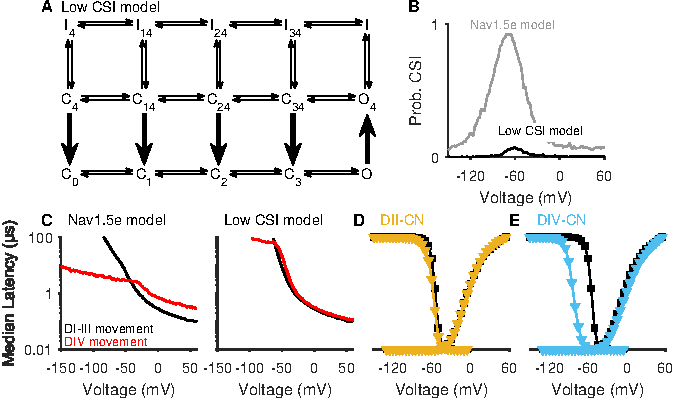
\includegraphics[width=115mm]{Figures/AppendixA/figure07.pdf}
% \end{minipage}\hfill
% \begin{minipage}[c]{60mm}
    \caption{\captiontitle{Closed-state inactivation determines consequences of voltage sensor neutralization.}
    (A) A schematic of the low CSI gating model. The thick black arrows represent the following parameter changes: rates $\alpha_4$ and $\beta_{4O}$ have been decreased 20-fold and rates $\alpha_{4O}$ and $\beta_4$ has been increased 20-fold, in an effort to bias the channel away from CSI and towards OSI.
    (B) The probability of CSI during voltage steps from -130 mV to voltages ranging from -130 to 60 mV, computed from 1000 stochastic simulations of the original Nav1.5e model (grey) and the low CSI model (black). The low CSI model has a significantly lower probability of CSI across all voltages.
    (C) Latencies were computed from the same simulations as panel B. Black lines represent the median latency until the Nav1.5e model (left) and low CSI model (right) reached the two rightmost columns of states, i.e. when DI-III had all moved. Red lines represent the median latency until the models reached the middle or top rows of states, i.e. latency to DIV movement.
    (D) The same manipulations for simulating DII-CN presented in \autoref{fig:A4} were applied to the low CSI model. In the low CSI model, DII-CN did not shift SSI significantly.
    (E) The same manipulations for simulating DIV-CN presented in \autoref{fig:A4} were applied to the low CSI model. This manipulation did not shift GV significantly.}
    \label{fig:A7}
% \end{minipage}
\end{figure}

\subsection{Neutralizing domain III and IV increases rate into closed-state inactivation}
At this point, all CN experimental results could be explained with Gating Scheme I, except for those associated with DIII-CN. The CN experiments suggest that, at least for Nav1.5, both DIII and DIV may be involved directly in inactivation, since their neutralization led to both a dramatic hyperpolarization of SSI and a decreased sensitivity of inactivation to changes in membrane potential. To investigate how the various domains, particularly DIII, contribute to the kinetics of inactivation, we measured the rate of recovery from inactivation for each CN mutant. An 80 ms pre-pulse to -10 mV was applied to inactivate all channels, followed by a -130 mV recovery pulse that lasted between 1 and 25 ms. Following this variable recovery interval, a test pulse to -10 mV was applied to determine the fraction of recovered channels (\autoref{fig:A8}A). Recovery curves were constructed by computing the peak current ratio between the pre-pulse and test pulse for each recovery interval (\autoref{fig:A8}B). This measurement revealed that neutralizing each domain slowed recovery from inactivation. To quantify these effects, recovery rate was estimated by fitting the curves with a biexponential function (Methods). This quantification confirmed that all mutants slowed the rate of recovery (\autoref{fig:A8}B).

\begin{figure}[t]
\begin{minipage}[c]{85mm}
    \centering
    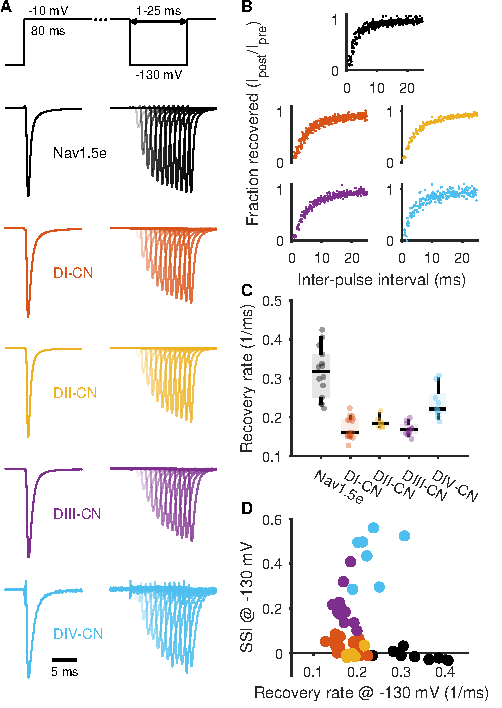
\includegraphics[width=\textwidth]{Figures/AppendixA/figure08.pdf}
\end{minipage}\hfill
\begin{minipage}[c]{70mm}
    \caption{\captiontitle{Neutralizing every voltage sensor in Nav1.5e slows recovery from inactivation.}
    (A) Top: voltage step protocol used to assess recovery from inactivation. Conditioning pulse of -10 mV was applied for 80 ms to inactivate channels before stepping to a variable length recovery pulse at -130 mV. After an inter-pulse interval ranging from 1-25 ms, a -10 mV test pulse was applied to assess the fraction of recovered channels. Bottom: representative traces of ionic currents through WT Nav1.5e and the four CN mutant channels.
    (B) Recovery curves of WT Nav1.5e and the four CN mutant channels. Colour scheme is the same as in panel A. Recovery curves were constructed by computing the ratio of peak currents evoked by the conditioning pulse to those evoked by the test pulse following each inter-pulse interval. All CN mutants display slower recovery curves.
    (C) Recovery rates were determined by fitting each recovery curve to the equation, $f\left(t\right)=A\exp{(\alpha_1t)}+\left(1-A\right)\exp{\left(\alpha_2t\right)}$ and was defined as $\alpha_w=A\alpha_1+\left(1-A\right)\alpha_2$. See \autoref{tab:AS1} for summary values.
    (D) The recovery rates determined from each cell are plotted against the amount of SSI at -130 mV. Even though all CN mutants have similar recovery rates at this potential, DIII- and DIV-CN display significantly more SSI.}
    \label{fig:A8}
\end{minipage}
\end{figure}

To determine how each mutant affects the rate into inactivation, we plotted the rate of recovery from inactivation against SSI measured at -130 mV (\autoref{fig:A8}D). At this voltage, DIII- and DIV-CN mutants displayed significantly more SSI than DI- and DII-CN mutants; however, they did not display slower rates of recovery from inactivation (\autoref{fig:A8}D). This observation indicates that the larger SSI shift from neutralizing DIII and DIV must result from accelerating the rate into inactivation. Since all SSI at this potential is CSI (\autoref{fig:A6}), we can conclude that the dramatic SSI shifts of DIII and DIV-CN mutants are largely a result of faster rates into CSI.

\subsection{Voltage-Clamp Fluorometry Reveals That Domains III and IV Are Necessary for Nav1.5 Inactivation}
One of the arguments for DIV sufficiency in inactivation is that neutralizing DIV in Nav1.4 leads to a shift in SSI that is so hyperpolarized, domains with intact voltage sensors must be in their deactivated state (Ahern et al., 2016; Capes et al., 2013). To test whether this is indeed the case for the neonatal Nav1.5 used in this study, we quantified the intrinsic voltage-sensitivity of each domain in Xenopus oocytes using VCF. Fluorescent probes were conjugated to each domain, thereby engineering four domain-tagged VCF constructs: DI*, DII*, DIII* and DIV*. Steady-state fluorescence was then measured at voltage steps ranging from -150 mV (-180 mV for DIII*) to 50 mV (\autoref{fig:A9}A-D).

\begin{figure}[t]
\begin{minipage}[c]{85mm}
    \centering
    \includegraphics[width=\textwidth]{Figures/AppendixA/figure09.pdf}
\end{minipage}\hfill
\begin{minipage}[c]{70mm}
    \caption{\captiontitle{Voltage-dependence of fluorescence from tagged voltage-sensing domains.}
    (A) Left: Representative fluorescence signals from a DI-tagged VCF construct (cell 20180510c2), recorded in Xenopus oocytes, in response to voltage steps of -140, -100, -60, -20 and +20 mV, shown by colour from darkest to lightest hue. Right: voltage-dependence of normalized fluorescence change from baseline (green circles). Solid green line is a fitted Boltzmann curve, parameters for which are reported in \autoref{tab:AS3}. Overlaid is the SSI (blue triangles) and GV curve (red inverted triangles) of WT Nav1.5e channels (\autoref{fig:A1} and \autoref{fig:A3}).  
    (B) Same as panel A, but for DII-tagged VCF constructs. (Representative traces from cell 20180512c1).  
    (C) Left: Representative traces for DIII-tagged VCF constructs (cell 20180518c4) in response to voltage steps of -180, -140, -100, -60, and -20 mV. Right: The dashed black line is the sum of the solid green line plus the derivative of the solid green line from panel D. 
    (D) Same as panel A, but for DIV-tagged VCF constructs. (Representative traces from cell 20180514c5). 
    (E) Left: Light blue circles represent the SSI curve from DIV-CN mutants (\autoref{fig:A3}) overlaid with the fluorescence-voltage relationship of VCF constructs DI*-DIII* (panels A-C). Right: fluorescence change from baseline plotted against the SSI curve of DIV-CN. Line of best fit for DIII* versus DIV-CN SSI is shown as dashes black line ($R^2 = 0.97$).
    \label{fig:A9}
}
\end{minipage}
\end{figure}

In agreement with other VCF studies of Nav1.5 channels, the fluorescence-voltage (F-V) curve for DI* was more hyperpolarized than that for DII* (\autoref{fig:A9}A, B) (Hsu et al., 2017; Varga et al., 2015). The voltage-dependence of the fluorescence signal of both DI* and DII* exhibited V\textsubscript{1/2} values of -65.4 ± 2.3 mV (n = 13) and -44.1 ± 0.7 mV (n = 17) (Q = 13.8, d.f. = 68, k = 4, $p < 10^{-5}$; Tukey’s range test), respectively, which were approximately 10 mV more depolarized than V\textsubscript{1/2} values reported for adult Nav1.5 channels (Hsu et al., 2017; Varga et al., 2015). This difference is in keeping with the more depolarized threshold for activation of Nav1.5e channels compared to the adult Nav1.5 splice variant (Onkal et al., 2008). Notably, the F-V plot of DII* had a shallower slope (k = 22.2 ± 0.6, n = 17) compared to DI* (k = 12.3 ± 1.2, n = 13) (Q = 11.5, $p < 10^{-5}$, d.f. = 68, k = 4; Tukey’s range test), indicating that DII has a lower sensitivity to changes in membrane potential.

The normalized F-V relationship for DIII* was significantly more hyperpolarized than DI* (Q = 45.2, $p < 10^{-5}$) and DII* (Q = 13.8, $p < 10^{-5}$) with a V\textsubscript{1/2} value of -137.4 ± 1.1 mV (n = 27) and a slope factor of 15.9 ± 0.6 (\autoref{fig:A9}C, D). Interestingly, the fluorescence signal was biphasic, reaching a maximum at about -50 mV and declining in intensity at more depolarized potentials (\autoref{fig:A9}C). This finding suggests that the voltage sensor of DIII may exhibit two distinct movements, analogous to the dynamics of the voltage sensor reported for Shaker K+-channels (Cha and Bezanilla, 1997) and DIII of Nav1.4 channels (Cha et al., 1999).

The F-V relationship observed for DIV* fluorescence occurred over a similar voltage range as SSI in WT channels (\autoref{fig:A9}D) in keeping with the role of this domain in inactivation. The V\textsubscript{1/2} value was -69.5 ± 1.3 mV (n=15) and the slope factor was 13.2 ± 0.5 mV. Interestingly, at potentials with observed DIV movement, the F-V relationship of DIII* deviates distinctly from a Boltzmann function. We observed that the fluorescence change of DIII was well fit by a Boltzmann function plus the derivative of the DIV* Boltzmann fit (\autoref{fig:A9}C). This observation seems to suggest an interaction between DIII and DIV movement, or between DIII and the binding of the inactivation motif. 

Finally, the voltage dependence of the F-V plot for DIII* was strongly correlated with measurements of SSI in DIV-CN mutants (\autoref{fig:A9}E). In fact, plotting the SSI of DIV-CN mutants versus the fluorescence signal of DIII* at each membrane potential displayed a strong linear correlation (\autoref{fig:A9}E). In contrast, the F-V curves for DI* and DII* were too depolarized to be correlated to SSI in DIV-CN mutants. This finding suggests that in the absence of DIV gating charges, DIII movement determines the voltage-dependence of SSI. Together with our previous results, this observation indicates that in Nav1.5, both DIII and DIV are intrinsically necessary for channel inactivation, whereas DI and DII are not.

\subsection{A structurally constrained Nav1.5 gating model}
To summarize all our results, we introduce Gating Scheme II (\autoref{fig:A10}A). In this modified model, both DIII and DIV must move prior to channel inactivation, as opposed to Gating Scheme I where DIV is sufficient for inactivation. Although we did not find direct evidence that DIII is necessary for pore opening, we kept the formalism from the first gating scheme, and made DI-III all necessary for pore opening. Another feature of Scheme II is that we have identified a specific domain order for the activation sequence. Whereas previously, DI-III moved in a nonspecific order prior to pore opening (\autoref{fig:A2}), here we identified the first transition with DIII, the second with DII, and the last with DI. This was motivated by several observations. The first being that DIII is active at much more negative voltages compared to DI and II (\autoref{fig:A9}B), making it likely that it would be first to activate during physiological changes in membrane potential. Additionally, DIII had the smallest effect on the peak G/V (\autoref{fig:A1}), suggesting that the domain contributes least to the rate of pore opening (\autoref{fig:A3}). Finally, because we found DI to be rate-limiting for pore opening (\autoref{fig:A3}), we made its activation the final step to pore opening. However, we note that these three domains are expected to activate in parallel (Chanda and Bezanilla, 2002), and stress that this sequential model is merely to reduce the complexity of the gating scheme. 

\begin{figure}[t]
\begin{minipage}[c]{85mm}
    \centering
    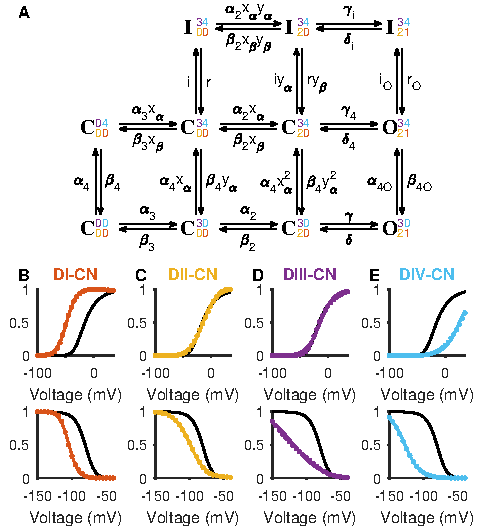
\includegraphics[width=\textwidth]{Figures/AppendixA/figure10.pdf}
\end{minipage}\hfill
\begin{minipage}[c]{70mm}
    \caption{\captiontitle{A new gating scheme where both DIII and DIV are necessary for inactivation.}
    (A) A kinetic model, referred to here as Gating Scheme II. The state $C_{00}^{00}$ represents the channel when all four voltage sensors are in their resting positions. The rightward transitions reflect the movement of the DIII voltage sensor, followed by DII, and finally DI. These three movements are sufficient to allow the channel to conduct. The transition from the bottom to middle row reflects DIV movement, while the transition from the middle to top row reflects binding of the inactivation motif. See main text for a full description of the model.
    (B) The GV (top) and SSI (bottom) curves of Gating Scheme II when parameterized with values reported in \autoref{tab:AS4} (black). See \autoref{fig:AS4} for a full comparison between model outcomes and Nav1.5e data. In red are the model outcomes when the charges associated with DI movement ($\gamma$, $\gamma_i$, $\gamma_4$, $\delta$, $\delta_i$, and $\delta_4$) were reduced and the intrinsic rates varied to reproduce DI-CN data. 
    (C) DII-CN mutant data were reproduced by targeting parameters $\alpha_2$ and $\beta_2$. 
    (D) DIII-CN mutant data were reproduced by targeting parameters $\alpha_3$ and $\beta_3$. 
    (E) DIV-CN mutant data were reproduced by targeting parameters $\alpha_4$, $\alpha_{4O}$, $\beta_4$, and $\beta_{4O}$. 
    Parameter values for all four CN models are reported in \autoref{tab:AS5}.
}
\label{fig:A10}
\end{minipage}
\end{figure}

Fitting the rate constants of Gating Scheme II to Nav1.5e data allowed the model to reproduce the channel’s activation, steady-state inactivation, and recovery from inactivation behaviour (\autoref{fig:AS4}, \autoref{tab:AS4}). In an attempt to capture the effects of VSD neutralization, we reduced the charge associated with each domain and re-fit the intrinsic rate of domain movement (\autoref{tab:AS5}). Modifying the transitions associated with each domain successfully reproduced the consequences of neutralizing each respective VSD (\autoref{fig:A10}B-E, c.f. \autoref{fig:A1} \& \autoref{fig:A5}).

Finally, we used this new model to investigate the difference between Nav1.5e and the adult form Nav1.5. The adult splice variant of Nav1.5 displays a G/V relationship that is 10 mV more hyperpolarized than Nav1.5e, while SSI and recovery are indistinguishable (Mancino et al., 2022). This difference results from two amino acid residues in DI which are thought to facilitate the translocation of DI-S4 in Nav1.5 (Mancino et al., 2022). Consistent with this, we found that to reproduce the behaviour of adult Nav1.5 with our model, it was sufficient to increase the forward rate of DI three-fold (\autoref{fig:A11}, \autoref{tab:AS5}). In conclusion, by identifying specific domains in the gating scheme, structurally-motivated parameter modifications were capable of replicating the consequences of neutralizing the various domains, as well as the gating differences between Nav1.5 splice variants.

\begin{figure}[t]
\begin{minipage}[c]{85mm}
    \centering
    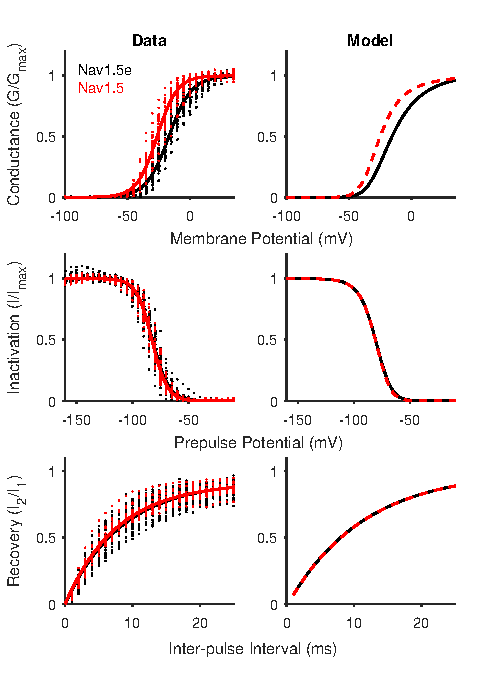
\includegraphics[width=\textwidth]{Figures/AppendixA/figure11.pdf}
\end{minipage}\hfill
\begin{minipage}[c]{70mm}
    \caption{\captiontitle{Manipulating intrinsic DI kinetics in the model reproduces difference between Nav1.5 and Nav1.5e.}
Left: Comparison of GV (top), SSI (middle), and recovery from inactivation (bottom) of Nav1.5e (black) and adult Nav1.5 (red). Solids lines represent Boltzmann fits. Data from Mancino et al. (2022).  Right: Output of Gating Scheme II fitted to Nav1.5e data (black) and after DI movement was facilitated by increasing rates $\gamma$ and $\gamma_i$ 3-fold (red). Exact parameter values for Nav1.5 model are presented in \autoref{tab:AS5}.}
\label{fig:A11}
\end{minipage}
\end{figure}

\section{Discussion}
We have studied the role of each voltage sensing domain, DI-IV, in Nav1.5 gating to investigate potential gating differences among Nav isoforms. We conclude that both DIII and DIV movements are necessary for Nav1.5 inactivation, unlike for Nav1.4, suggesting that cardiac sodium channels follow a different gating scheme from skeletal muscle sodium channels. Additionally, our results suggest that high levels of closed-state inactivation (CSI) permit all voltage sensors to influence inactivation, while low levels of CSI restrict each voltage sensor to influence either activation or inactivation. We postulate that the distinct propensities for CSI displayed by Nav1.4, Nav1.5, and Nav1.6 channels allow the same voltage sensors to shape macroscopic gating properties differently in each channel.

\subsection{Contributions of voltage sensing domains to pore opening}
Previous charge neutralization experiments have reported disparate changes to the voltage-dependence of activation when comparing skeletal muscle (Capes et al., 2013; Chahine et al., 1994), neuronal (Kontis and Goldin, 1997), and cardiac (Chen et al., 1996) Nav channels. Here, we showed that changes to GV curves is an unreliable marker for a domain’s role in activation, whereas the latency to peak current is more informative (\autoref{fig:A3} \& \ref{fig:A4}). Using this measure, we found that in the neonatal sodium channel, Nav1.5e, DI movement is likely rate limiting for pore opening and DII movement contributes significantly, but to a lesser degree. Although DIII movement is thought to be necessary for channel activation in Nav1.4 skeletal muscle channels (Chanda and Bezanilla, 2002), neutralizing DIII in Nav1.5 did not alter the voltage dependence or kinetics of channel activation (\autoref{fig:A1} \& \ref{fig:A2}). This is likely because DIII is already in its activated position in wildtype Nav1.5 channels at the voltage range used in our protocols (\autoref{fig:A5}) (Hsu et al., 2017; Zhu et al., 2017). Consequently, neutralizing the domain’s voltage sensor would not be expected to significantly alter the overall activation process. Finally, although DIV-CN Nav1.5 mutants exhibit an altered voltage-dependence of activation, the observed effects are more consistent with an increased inactivation rate (\autoref{fig:A3}F). Considering this, we did not find evidence that DIV movement is necessary for activation, consistent with previous experiments on Nav1.4 channels that were mutated to prevent inactivation (Goldschen-Ohm et al., 2013). In summary, our results suggest that DI, and to a lesser extent DII, determines the rate of activation, whereas DIII, at least in Nav1.5, likely plays little role in activation at physiological membrane potentials.

\subsection{All voltage sensors contribute to Nav channel inactivation}
Charge-neutralization experiments on Nav1.4 have suggested that DIV is uniquely sufficient for inactivation (Capes et al., 2013). Here, we found that neutralizing either DIII or DIV leads to a similar hyperpolarizing shift and flattening of the SSI curve. Furthermore, we observed that SSI in DIV-CN Nav1.5 mutants is strongly correlated with DIII movement (\autoref{fig:A5}E). Together, this suggests that Nav1.5 inactivation is intrinsically coupled to DIII movement. Our results contrast with those of Cha et al. (1996), whose charge neutralization experiments on Nav1.5 identified a unique role for DIV in inactivation. Our experiments differ from those of Cha et al. in that we neutralized the first three gating charges of each domain, whereas they neutralized one charge at a time. It is therefore likely that the majority of gating charge for DIV is contributed by a single arginine, as previously suggested (Cha et al., 1996), while DIII gating charge is contributed more uniformly by the entire S4 sensor. 

Notably, DIV-CN Nav1.4 mutants inactivate at voltages too hyperpolarized to be caused by the movement of DIII (Chanda and Bezanilla, 2002; Capes et al., 2013), and DIII-CN Nav1.4 mutants do not display significantly altered SSI (Capes et al., 2013). Both of these observations are starkly different from our measurements of Nav1.5 (\autoref{fig:A5} \& \ref{fig:A9}). Accordingly, we conclude that DIII is coupled to inactivation differently in Nav1.4 and Nav1.5 channels, which could contribute to the divergent views surrounding the role of DIII in inactivation (Ahern et al., 2016; Armstrong and Hollingworth, 2018). Our results do, however, support the idea that DIV movement is rate-limiting for inactivation (Capes et al., 2013). This follows from the fact that DIV-CN depolarized activation in our experiments without altering time to peak current, indicating that neutralizing DIV accelerates the rate of CSI (\autoref{fig:A3} \& \ref{fig:A4}).

Finally, although we found that neutralizing DI and DII significantly affects Nav1.5 inactivation, these observations could be explained by coupling between channel activation and inactivation (Kuo and Bean, 1994), a feature also assumed about Nav1.4 gating (Capes et al., 2013). Therefore, discrepancies between neutralizing DI and DII in Nav1.4 and Nav1.5 are probably not from their separate gating schemes, per se. As explained below, we postulate that the variable contributions of DI and DII to SSI is a result of differing intrinsic propensities for CSI among Nav isoforms.

\subsection{Closed-state inactivation is variable among different Nav channel isoforms}
It is well established that Nav channels can inactivate from closed states (Aldrich et al., 1983; Armstrong, 2006; Bean, 1981; Lawrence et al., 1991; Vandenberg and Horn, 1984), which is thought to occur when DIII and DIV (possibly just DIV in Nav1.4) move prior to channel activation (Armstrong, 2006). Nevertheless, the prevailing idea is that DIV movement is substantially slower than the other domains across all voltages (Armstrong, 2006; Bosmans et al., 2008; Capes et al., 2013; Chanda and Bezanilla, 2002), implying that inactivation occurs predominantly from the open state. Our findings on Nav1.5 seem to contradict this view. Indeed, the effects of DI- \& DII-CN on SSI (\autoref{fig:A5}), the effects of DIV-CN on the G/V relationship (\autoref{fig:A1}), and the high levels of CSI that turn entirely to OSI at more depolarized potentials (\autoref{fig:A6}) all strongly indicate that the order of domain movements is governed by the relative dynamics of each voltage sensor, and not by a fixed sequence of movements. We, in fact, conclude that DIV moves faster than DI-III at a large range of voltages.

It should be noted that we performed our CN experiments in HEK293 cells with mouse Nav1.5e expressed alone, whereas the same experiments by Capes et al. (2013) were performed in oocytes on rat Nav1.4 channels co-expressed with $\beta_1$ auxiliary subunits. Interestingly, past VCF experiments revealing slow DIV movement were also performed in oocytes in the presence of $\beta$ subunits, on either human Nav1.4 (Cha et al., 1999) or rat Nav1.4 (Chanda and Bezanilla, 2002). This could point to intrinsic differences in activation sequences among Nav isoforms, as suggested by the different levels of CSI measured from Nav1.4, Nav1.5, and Nav1.6 (\autoref{fig:A6}). However, it will be important to determine whether the dynamics of each domain are also affected by expression system, sequence differences among Nav paralogs, and/or the presence of beta subunits. 

The idea that CSI is variable has some interesting implications. Our results suggest that a high propensity for CSI permits DI and DII to alter SSI and also allows DIV to alter the voltage dependence of activation (\autoref{fig:A1}-\ref{fig:A7}). Intriguingly, many gating modifiers influence channel behaviour by targeting the movement of specific voltage sensors, and may thus have CSI-dependent effects. Several studies on toxins that target voltage sensors --- which include certain scorpion, sea anemone, and cone snail toxins (Ahern et al., 2016) --- have described varied effects across Nav channel isoforms (Alami et al., 2003; Leipold et al., 2006; Oliveira et al., 2004). Furthermore, auxiliary $\beta$ subunits target specific voltage sensing domains (Zhu et al., 2017), and have variable effects on Nav1.4 and Nav1.5 (Bendahhou et al., 1995; Zhu et al., 2017; Malhotra et al., 2001; Nuss et al., 1995; Ferrera and Moran, 2006). It has been suggested that some of these observations result from steric effects of channel structure (Alami et al., 2003; Jiang et al., 2020). Our findings suggest that differences in channel dynamics, specifically as they pertain to CSI, may also contribute to these variable effects of Nav channel modifiers. We predict that channels with a low propensity for CSI may be less susceptible to gating modulation. 

Finally, with respect to channel mutations, it has been suggested that insights into channelopathies may be realized through the analysis of “homologous” mutations across Nav channels (Loussouarn et al., 2016). Whether variation in gating kinetics alter the consequences of other mutations as profoundly as those of the voltage sensor neutralizing mutations studied here is clearly of interest for future study.

\section{Acknowledgments}

We thank Dr. Mark Aurousseau who cloned Nav1.5e from brain extracts and Dr. Jonathan R. Silva for the gift of Nav1.5 voltage-clamp fluorometry cDNA constructs. We also thank members of the Bowie laboratory, for discussions and comments on the manuscript.

\noindent \textbf{Funding}: This work was supported by Canadian Institutes of Health Research Operating Grants CIHR MOP-342247 to D.B, by the Natural Sciences and Engineering Council of Canada Discovery Grant to A.K., and by JSPS KAKENHI grants 17H04021 and 20H03424 to Y.K. N.B. was supported by the NSERC-CREATE in Complex Dynamics Graduate Scholarship. A.S.M. was supported by the NSERC CGS-Master’s Scholarship. 

\noindent \textbf{Author contributions}: 
Conceptualization: NB, ASM, and DB
Methodology: NB, TS, and YK
Formal Analysis: NB, ASM, YY, and TS
Investigation: NB, ASM, and YY
Writing – Original Draft: NB and DB
Writing – Review \& Editing: all authors
Visualization: NB
Supervision: AK and DB
Project Administration, DB
Funding Acquisition: YK, AK, and DB

\noindent \textbf{Competing interests}: Authors declare that they have no competing interests.

\section{References}


\begin{hangparas}{.25in}{1}
Ahern, C.A., J. Payandeh, F. Bosmans, and B. Chanda. 2016. The hitchhiker’s guide to the voltage-gated sodium channel galaxy. J. Gen. Physiol. 147:1–24. \url{doi:10.1085/jgp.201511492}.

Ahier, A., and S. Jarriault. 2014. Simultaneous Expression of Multiple Proteins Under a Single Promoter in Caenorhabditis elegans via a Versatile 2A-Based Toolkit. Genetics. 196:605–613. \url{doi:10.1534/genetics.113.160846}.

Alami, M., H. Vacher, F. Bosmans, C. Devaux, J.P. Rosso, P.E. Bougis, J. Tytgat, H. Darbon, and M.F. Martin-Eauclaire. 2003. Characterization of Amm VIII from Androctonus mauretanicus mauretanicus: A new scorpion toxin that discriminates between neuronal and skeletal sodium channels. Biochem. J. 375:551–560. \url{doi:10.1042/BJ20030688}.

Aldrich, R.W., D.P. Corey, and C.F. Stevens. 1983. A reinterpretation of mammalian sodium channel gating based on single channel recording. Nature. 306:436–41. \url{doi:10.1038/306436a0}.

Angsutararux, P., P.W. Kang, W. Zhu, and J.R. Silva. 2021. Conformations of voltage-sensing domain iii differentially define nav channel closed-and open-state inactivation. J. Gen. Physiol. 153:1–11. \url{doi:10.1085/jgp.202112891}.

Armstrong, C.M. 2006. Na channel inactivation from open and closed states. Proc. Natl. Acad. Sci. 103:17991–17996. \url{doi:10.1073/pnas.0607603103}.

Armstrong, C.M., and S. Hollingworth. 2018. A perspective on Na and K channel inactivation. J. Gen. Physiol. 150:7–18. \url{doi:10.1085/jgp.201711835}.

Bean, B.P. 1981. Sodium channel inactivation in the crayfish giant axon. Must channels open before inactivating? Biophys. J. 35:595–614. \url{doi:10.1016/S0006-3495(81)84815-1}.

Bendahhou, S., T.R. Cummins, J.F. Potts, J. Tong, and W.S. Agnew. 1995. Serine-1321-independent regulation of the $\mu$1 adult skeletal muscle Na+ channel by protein kinase C. Proc. Natl. Acad. Sci. U. S. A. 92:12003–12007. \url{doi:10.1073/pnas.92.26.12003}.

Bosmans, F., M.-F. Martin-Eauclaire, and K.J. Swartz. 2008. Deconstructing voltage sensor function and pharmacology in sodium channels. Nature. 456:202–208. \url{doi:10.1038/nature07473}.

Braman, J., C. Papworth, and A. Greener. 1996. Site-directed mutagenesis using double-stranded plasmid DNA templates. In Methods in molecular biology (Clifton, N.J.).

Camacho, J.A., S. Hensellek, J.-S. Rougier, S. Blechschmidt, H. Abriel, K. Benndorf, and T. Zimmer. 2006. Modulation of Na v 1.5 Channel Function by an Alternatively Spliced Sequence in the DII/DIII Linker Region. J. Biol. Chem. 281:9498–9506. \url{doi:10.1074/jbc.M509716200}.

Capes, D.L., M.P. Goldschen-Ohm, M. Arcisio-Miranda, F. Bezanilla, and B. Chanda. 2013. Domain IV voltage-sensor movement is both sufficient and rate limiting for fast inactivation in sodium channels. J. Gen. Physiol. 142:101–112. \url{doi:10.1085/jgp.201310998}.

Catterall, W.A., A.L. Goldin, and S.G. Waxman. 2005. International Union of Pharmacology. XLVII. Nomenclature and Structure-Function Relationships of Voltage-Gated Sodium Channels. Pharmacol. Rev. 57:397–409. \url{doi:10.1124/pr.57.4.4}.

Catterall, W.A., G. Wisedchaisri, and N. Zheng. 2020. The conformational cycle of a prototypical voltage-gated sodium channel. Nat. Chem. Biol. 16:1314–1320. \url{doi:10.1038/s41589-020-0644-4}.

Cha, A., and F. Bezanilla. 1997. Characterizing Voltage-Dependent Conformational Changes in the ShakerK+ Channel with Fluorescence. Neuron. 19:1127–1140. \url{doi:10.1016/S0896-6273(00)80403-1}.

Cha, A., P.C. Ruben, A.L. George, E. Fujimoto, and F. Bezanilla. 1999. Voltage sensors in domains III and IV, but not I and II, are immobilized by Na+ channel fast inactivation. Neuron. 22:73–87. \url{doi:10.1016/S0896-6273(00)80680-7}.

Chahine, M., A.L. George, M. Zhou, S. Ji, W. Sun, R.L. Barchi, and R. Horn. 1994. Sodium channel mutations in paramyotonia congenita uncouple inactivation from activation. Neuron. 12:281–294. \url{doi:10.1016/0896-6273(94)90271-2}.

Chanda, B., and F. Bezanilla. 2002. Tracking voltage-dependent conformational changes in skeletal muscle sodium channel during activation. J. Gen. Physiol. 120:629–645. \url{doi:10.1085/jgp.20028679}.

Chen, L.Q., V. Santarelli, R. Horn, and R.G. Kallen. 1996. A unique role for the S4 segment of domain 4 in the inactivation of sodium channels. J. Gen. Physiol. 108:549–556. \url{doi:10.1085/jgp.108.6.549}.

Edelheit, O., A. Hanukoglu, and I. Hanukoglu. 2009. Simple and efficient site-directed mutagenesis using two single-primer reactions in parallel to generate mutants for protein structure-function studies. BMC Biotechnol. 9:61. \url{doi:10.1186/1472-6750-9-61}.

Ferrera, L., and O. Moran. 2006. $\beta1$-subunit modulates the Nav1.4 sodium channel by changing the surface charge. Exp. Brain Res. 172:139–150. \url{doi:10.1007/s00221-005-0323-4}.

Goldschen-Ohm, M.P., D.L. Capes, K.M. Oelstrom, and B. Chanda. 2013. Multiple pore conformations driven by asynchronous movements of voltage sensors in a eukaryotic sodium channel. Nat. Commun. 4:1310–1350. \url{doi:10.1038/ncomms2356}.

Hsu, E.J., W. Zhu, A.R. Schubert, T. Voelker, Z. Varga, and J.R. Silva. 2017. Regulation of Na+ channel inactivation by the DIII and DIV voltage-sensing domains. J. Gen. Physiol. 149:389–403. \url{doi:10.1085/jgp.201611678}.

Hull, J.M., and L.L. Isom. 2018. Voltage-gated sodium channel $\beta$ subunits: The power outside the pore in brain development and disease. Neuropharmacology. 132:43–57. \url{doi:10.1016/j.neuropharm.2017.09.018}.

Jiang, D., H. Shi, L. Tonggu, T.M. Gamal El-Din, M.J. Lenaeus, Y. Zhao, C. Yoshioka, N. Zheng, and W.A. Catterall. 2020. Structure of the Cardiac Sodium Channel. Cell. 180:122-134.e10. \url{doi:10.1016/j.cell.2019.11.041}.

Jordan, M., A. Schallhorn, and F.M. Wurm. 1996. Transfecting Mammalian Cells: Optimization of Critical Parameters Affecting Calcium-Phosphate Precipitate Formation. Nucleic Acids Res. 24:596–601. \url{doi:10.1093/nar/24.4.596}.

Kontis, K.J., and A.L. Goldin. 1997. Sodium channel inactivation is altered by substitution of voltage sensor positive charges. J. Gen. Physiol. 110:403–413. \url{doi:10.1085/jgp.110.4.403}.

Kühn, F.J.P., and N.G. Greeff. 1999. Movement of Voltage Sensor S4 in Domain 4 Is Tightly Coupled to Sodium Channel Fast Inactivation and Gating Charge Immobilization. J. Gen. Physiol. 114:167–184. \url{doi:10.1085/jgp.114.2.167}.

Kume, S., T. Shimomura, M. Tateyama, and Y. Kubo. 2018. Two mutations at different positions in the CNBH domain of the hERG channel accelerate deactivation and impair the interaction with the EAG domain. J. Physiol. 596:4629–4650. \url{doi:10.1113/JP276208}.

Kuo, C.-C., and B.P. Bean. 1994. Na+ channels must deactivate to recover from inactivation. Neuron. 12:819–829. \url{doi:10.1016/0896-6273(94)90335-2}.

Lawrence, J.H., D.T. Yue, W.C. Rose, and E. Marban. 1991. Sodium channel inactivation from resting states in guinea-pig ventricular myocytes. J. Physiol. 443:629–650. \url{doi:10.1113/jphysiol.1991.sp018855}.

Leipold, E., A. Hansel, A. Borges, and S.H. Heinemann. 2006. Subtype specificity of scorpion $\beta$-toxin Tz1 interaction with voltage-gated sodium channels is determined by the pore loop of domain 3. Mol. Pharmacol. 70:340–347. \url{doi:10.1124/mol.106.024034}.

Loussouarn, G., D. Sternberg, S. Nicole, C. Marionneau, F. Le Bouffant, G. Toumaniantz, J. Barc, O.A. Malak, V. Fressart, Y. Péréon, I. Baró, and F. Charpentier. 2016. Physiological and Pathophysiological Insights of Nav1.4 and Nav1.5 Comparison. Front. Pharmacol. 6. \url{doi:10.3389/fphar.2015.00314}.

Malhotra, J.D., C. Chen, I. Rivolta, H. Abriel, R. Malhotra, L.N. Mattei, F.C. Brosius, R.S. Kass, and L.L. Isom. 2001. Characterization of sodium channel $\alpha$- and $\beta$-subunits in rat and mouse cardiac myocytes. Circulation. 103:1303–1310. \url{doi:10.1161/01.CIR.103.9.1303}.

Mancino, A.S., W.G. Glass, Y. Yan, P.C. Biggin, and D. Bowie. 2022. Spliced isoforms of the cardiac Nav1.5 channel modify channel activation by distinct structural mechanisms. J. Gen. Physiol. 154:1–17. \url{doi:10.1085/jgp.202112906}.

Mitrovic, N., A.L. George, and R. Horn. 1998. Independent versus coupled inactivation in sodium channels role of the domain 2 S4 segment. J. Gen. Physiol. 111:451–462. \url{doi:10.1085/jgp.111.3.451}.

Nuss, H.B., N. Chiamvimonvat, M.T. Pérez-García, G.F. Tomaselli, and E. Marbán. 1995. Functional association of the $\beta1$ subunit with human cardiac (hH1) and rat skeletal muscle ($\mu$1) sodium channel $\alpha$ subunits expressed in Xenopus oocytes. J. Gen. Physiol. 106:1171–1191. \url{doi:10.1085/jgp.106.6.1171}.

Oliveira, J.S., E. Redaelli, A.J. Zaharenko, R.R. Cassulini, K. Konno, D.C. Pimenta, J.C. Freitas, J.J. Clare, and E. Wanke. 2004. Binding specificity of sea anemone toxins to Nav 1.1-1.6 sodium channels. Unexpected contributions from differences in the IV/S3-S4 outer loop. J. Biol. Chem. 279:33323–33335. \url{doi:10.1074/jbc.M404344200}.

Onkal, R., J.H. Mattis, S.P. Fraser, J.K.J. Diss, D. Shao, K. Okuse, and M.B.A. Djamgoz. 2008. Alternative splicing of Nav1.5: An electrophysiological comparison of “neonatal” and “adult” isoforms and critical involvement of a lysine residue. J. Cell. Physiol. 216:716–726. \url{doi:10.1002/jcp.21451}.

Pan, X., Z. Li, Q. Zhou, H. Shen, K. Wu, X. Huang, J. Chen, J. Zhang, X. Zhu, J. Lei, W. Xiong, H. Gong, B. Xiao, and N. Yan. 2018. Structure of the human voltage-gated sodium channel Na v 1.4 in complex with $\beta1$. Science. 362:eaau2486. \url{doi:10.1126/science.aau2486}.

Vandenberg, C.A., and R. Horn. 1984. Inactivation viewed through single sodium channels. J. Gen. Physiol. 84:535–64. \url{doi:10.1085/jgp.84.4.535}.

Varga, Z., W. Zhu, A.R. Schubert, J.L. Pardieck, A. Krumholz, E.J. Hsu, M.A. Zaydman, J. Cui, and J.R. Silva. 2015. Direct Measurement of Cardiac Na + Channel Conformations Reveals Molecular Pathologies of Inherited Mutations. Circ. Arrhythmia Electrophysiol. 8:1228–1239. \url{doi:10.1161/CIRCEP.115.003155}.

Zhu, W., T.L. Voelker, Z. Varga, A.R. Schubert, J.M. Nerbonne, and J.R. Silva. 2017. Mechanisms of noncovalent $\beta$ subunit regulation of NaV channel gating. J. Gen. Physiol. 149:813–831. \url{doi:10.1085/jgp.201711802}.
\end{hangparas}

\clearpage

\renewcommand{\thefigure}{A.S\arabic{figure}}
\renewcommand{\figurename}{Supplementary Fig.}
\setcounter{figure}{0}

\renewcommand{\thetable}{A.S\arabic{table}}
\renewcommand{\tablename}{Supplementary Table}
\setcounter{table}{0}

\section{Supplementary information}

\subsection{Supplementary figures}

\centerline{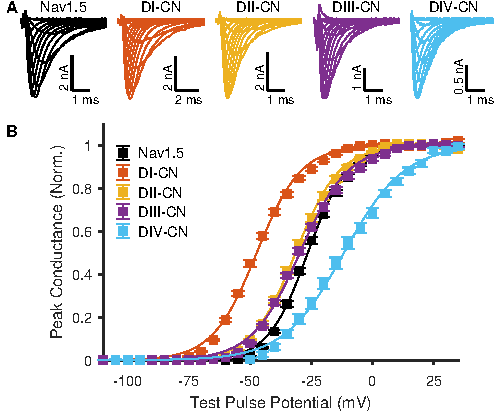
\includegraphics[width=85mm]{Figures/AppendixA/figureS1.pdf}}
\centerline{
\begin{minipage}[c]{\textwidth}
\captionof{figure}{\captiontitle{Changes in peak GV following domain neutralization in adult form of Nav1.5, mH1.} Related to \autoref{fig:A1}.
(A) Representative traces of ionic currents corresponding to wild-type (WT) Nav1.5 (cell 20170311c3) and mutant channels (DI-CN, cell 20180301c6; DII-CN, cell 20180711c3; DIII-CN, cell 20180309c12; DIV-CN, cell 20181022c7) in response to depolarizing voltage steps ranging from -110 to 35 mV, following a holding potential of -130 mV (-100 mV for WT), recorded in HEK-293T cells. 
(B) Summary data corresponding to panel A, showing normalized peak current following the test pulse, as a function of the test pulse voltage.} 
\label{fig:AS1}
\end{minipage}
}
\newpage


\centerline{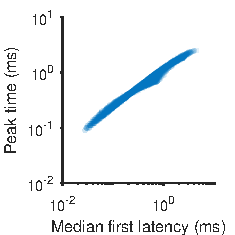
\includegraphics[width=45mm]{Figures/AppendixA/figureS2.pdf}}
\centerline{
\begin{minipage}[c]{\textwidth}
\captionof{figure}{\captiontitle{Correlation between time to peak current and latency to first channel opening in Nav1.5e gating model.}  Related to \autoref{fig:A3}.
Gating Scheme I was simulated with different parameter combinations. Both the rate $\alpha$ and the rates $\gamma$, $\gamma_i$, and $\gamma_4$ were varied from 10-fold less to 10-fold more than their fitted values (\autoref{tab:AS2}). The median first open latency across 1000 stochastic simulations is plotted against the peak time of the macroscopic current for each parameter combination. } 
\label{fig:AS2}
\end{minipage}
}
\newpage


\centerline{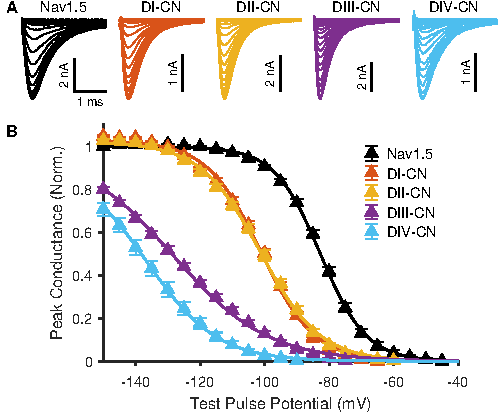
\includegraphics[width=85mm]{Figures/AppendixA/figureS3.pdf}}
\centerline{
\begin{minipage}[c]{\textwidth}
\captionof{figure}{\captiontitle{Changes in steady-state inactivation following domain neutralization in adult form of Nav1.5, mH1.} Related to \autoref{fig:A3}.
(A) Representative traces of ionic currents corresponding to wild-type (WT) Nav1.5 (cell 20170311c3) and mutant channels (DI-CN, cell 20180301c6; DII-CN, cell 20180711c3; DIII-CN, cell 20180309c12; DIV-CN, cell 20190305c4) in response to a test pulse to -10 mV following conditioning pulses ranging from -160 to -30 mV. 
(B) Summary data corresponding to panel A, showing normalized peak current following the test pulse, as a function of the conditioning pulse voltage.}
\label{fig:AS3}
\end{minipage}
}
\newpage


\centerline{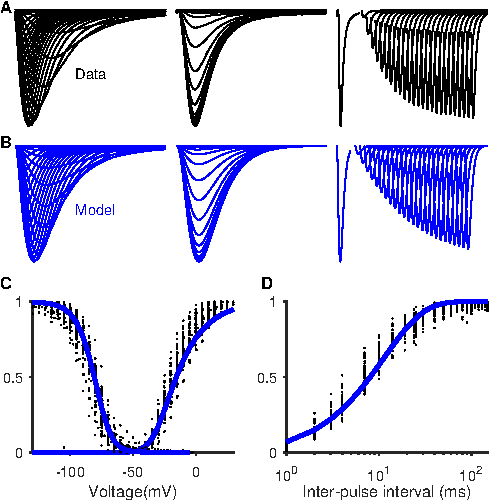
\includegraphics[width=85mm]{Figures/AppendixA/figureS4.pdf}}
\centerline{
\begin{minipage}[c]{\textwidth}
\captionof{figure}{\captiontitle{Gating Scheme II fitted to Nav1.5e data.} Related to \autoref{fig:A9} and \ref{fig:A10}.
Description of each panel is the same as in \autoref{fig:A2}. Here, blue is the model output of Gating Scheme II (\autoref{fig:A9}) parameterized with the values presented in \autoref{tab:AS4}. Black traces represent experimental data collected on Nav1.5e.} 
\label{fig:AS4}
\end{minipage}
}
\newpage

\subsection{Supplementary tables}

\noindent
% \setlength{\tabcolsep}{2pt}
\begin{minipage}{\linewidth}
    \captionof{table}{\captiontitle{Boltzmann parameters for Nav1.5e. Related to \autoref{fig:A1}, \ref{fig:A5}, and \ref{fig:A7}.}}
    \label{tab:AS1}
    \vskip-\abovecaptionskip
    \vskip+\belowcaptionskip
    \small
    \begin{tabular}{l|rrr|rrr|rr}
    \hiderowcolors
        \hline
        & \multicolumn{3}{c|}{Activation} & \multicolumn{3}{c|}{Steady-state inactivation} & \multicolumn{2}{c}{Recovery from inactivation} \\
        & V\textsubscript{1/2} (mV) & k (mV) & n & V\textsubscript{1/2} (mV) & k (mV) & n & $a_w$ (1/ms) & n \\
        \hline
        WT & -16.8 ± 0.5 & 9.0 ± 0.1   & 51 & -82.0 ± 0.5    & -7.2 ± 0.1   & 49 &  0.31 ± 0.02 & 14 \\
        DI-CN & -48.1 ± 0.6 & 9.9 ± 0.1   & 24 & -100.9 ± 0.5   & -8.7 ± 0.1   & 23 &  0.17 ± 0.01 & 16 \\
        DII-CN & -22.6 ± 0.5 & 9.6 ± 0.2   & 26 & -96.5 ± 0.8    & -9.2 ± 0.2   & 25 &  0.19 ± 0.01 & 7 \\
        DIII-CN & -19.0 ± 0.6 & 10.3 ± 0.2  & 23 & -120.0 ± 1.1   & -14.4 ± 0.2  & 23 &  0.17 ± 0.01 & 11 \\
        DIV-CN & -7.4 ± 1.3  & 10.7 ± 0.3  & 14 & -131.1 ± 2.6   & -13.7 ± 1.5  & 13 &  0.24 ± 0.01 & 9 \\
        
        \hline
    \end{tabular}    
    \vskip-\abovecaptionskip
    \vskip+\belowcaptionskip
    \singlespacing
    \footnotesize
    \begin{flushleft}
        Estimated Boltzmann parameters, $V_{1/2}$ and k, from fitting the equation, $f\left(V\right)=\left[1+\exp{\left(-\frac{V-V_{1/2}}{k}\right)}\right]^{-1}$, to peak activation (G/V) curves (\autoref{fig:A1}) and steady-state inactivation (SSI) curves (\autoref{fig:A4}). n is the number of samples. Recovery rate was determined from fitting recovery curve (\autoref{fig:A7}) to the equation, $f\left(t\right)=A\exp{(\alpha_1t)}+\left(1-A\right)\exp{\left(\alpha_2t\right)}$ and was defined as $\alpha_w=A\alpha_1+\left(1-A\right)\alpha_2$. Data report mean ± SEM.  
    \end{flushleft}
\end{minipage}

\vspace{1em}

\noindent
\begin{minipage}{\linewidth}
    \captionof{table}{\captiontitle{Parameters for Gating Scheme I that reproduce Nav1.5e data. Related to \autoref{fig:A2}.}} 
    \label{tab:AS2}
    \vskip-\abovecaptionskip
    \vskip+\belowcaptionskip
    \small
    \begin{tabular}{lrrrr}
    \hiderowcolors
        \hline
        Rate Constant & $k^*$ & q & \multicolumn{2}{c}{Cooperativity Factor} \\
        \hline
        $\alpha$   &   15700   &  0.26 &  $x_\alpha$ & 0.86 \\
        $\alpha_{4}$  &  506      &  0.32 &  $x_\beta$ & 0.049 \\
        $\alpha_{4o}$ & 1620      &  0.32 &  $y_\alpha$ & 3.7 \\
        $\beta$   &   985     & -1.3  &  $y_\beta$ & 0.8 \\
        $\beta_{4}$  &  252000   & -0.48 &     & \\
        $\beta_{4o}$ & 98.4      & -0.48 &     & \\
        $\delta$   &   775     & -2.3  &     & \\
        $\delta_4$  &  880      & -2.3  &     & \\
        $\delta_i$  &  135      & -2.3  &     & \\
        $\gamma$   &   9060    &  1.5  &     & \\
        $\gamma_4$  &  15300    &  1.5  &     & \\
        $\gamma_i$  &  5370     &  1.5  &     & \\
        $i$   &   24200   &    0  &     & \\
        $i_o$  &  9880     &    0  &     & \\
        $r$   &   2630    &    0  &     & \\
        $r_o$  &  4.8      &    0  &     & \\

        \hline
    \end{tabular}    
    \vskip-\abovecaptionskip
    \vskip+\belowcaptionskip
    \singlespacing
    \footnotesize
    \begin{flushleft}
        The rate, $k$, of each transition is computed as $k = k^* \exp(qV/KT)$, where $V$ is the membrane voltage, $K$ is Boltzmann’s constant, $T$ is the temperature, and $k^*$ and $q$ are fitted parameters (see Methods). The rates $\gamma_4^*$ and $r^*$ were dependent on the other parameters such that microscopic reversibility was enforced. The charge associated with $i$, $i_o$, $r$, and $r_o$ were all constrained to be zero. The charges associated with $\gamma_4$, $\gamma$, and $\gamma_i$ were defined to be the same. Likewise, the charges for $\delta_4$, $\delta$, and $\delta_i$.
    \end{flushleft}
\end{minipage}


\noindent
\begin{minipage}{\linewidth}
    \captionof{table}{\captiontitle{Boltzmann parameters for fluorescence-voltage (F-V) curves. Related to \autoref{fig:A8}.}}
    \label{tab:AS3}
    \vskip-\abovecaptionskip
    \vskip+\belowcaptionskip
    \small
    \begin{tabular}{lrrr}
    \hiderowcolors
        \hline
        \multicolumn{1}{c}{Nav1.5e}     & \multicolumn{1}{c}{V\textsubscript{1/2}}  &  \multicolumn{1}{c}{k} &  \multicolumn{1}{c}{n} \\
        \hline
        DI*-VCF     & -65.4 ± 2.3   & 12.3 ± 1.2  & 13 \\
        DII*-VCF    & -44.1 ± 0.7   & 22.2 ± 0.6  & 17 \\
        DIII*-VCF   & -137.4 ± 1.1  & 15.9 ± 0.6  & 27 \\
        DIV*-VCF    & -69.5 ± 1.3   & 13.2 ± 0.5  & 15 \\
        \hline
    \end{tabular} 

\end{minipage}

\vspace{1em}

\noindent
\begin{minipage}{\linewidth}
    \captionof{table}{\captiontitle{Parameters for Gating Scheme II that reproduce Nav1.5e data. Related to \autoref{fig:AS4}.}} 
    \label{tab:AS4}
    \vskip-\abovecaptionskip
    \vskip+\belowcaptionskip
    \small
    \begin{tabular}{lrrrr}
    \hiderowcolors
        \hline
        Rate Constant & $k^*$ & q & \multicolumn{2}{c}{Cooperativity Factor} \\
        \hline
        $\alpha_{2}$    &   8640    &   0.35    &     $x_\alpha$    &   0.87    \\
        $\alpha_{3}$    &   5240    &   0.39    &     $x_\beta$     &   0.03    \\
        $\alpha_{4}$    &   1590    &   0.47    &     $y_\alpha$    &   3.3 \\
        $\alpha_{4o}$   &   2330    &   0.47    &     $y_\beta$     &   0.82    \\
        $\beta_{2}$     &   1020    &   -2.1    &       &        \\
        $\beta_{3}$     &   209 &   -1.8    &           &        \\
        $\beta_{4}$     &   18400   &   -0.21   &           &        \\
        $\beta_{4o}$    &   178 &   -0.21   &           &        \\
        $\delta$    &   183 &   -1.6    &           &        \\
        $\delta_4$      &   880 &   -1.6    &           &        \\
        $\delta_i$      &   12.8    &   -1.6    &           &        \\
        $\gamma$    &   6960    &   1.3 &           &        \\
        $\gamma_i$      &   2340    &   1.3 &           &        \\
        $i$     &   37900   &   0   &           &        \\
        $i_o$   &   3620    &   0   &           &       \\
        $r$     &   573 &   0   &       &       \\
        \hline
    \end{tabular}    
\end{minipage}


\noindent
\begin{minipage}{\linewidth}
    \captionof{table}{\captiontitle{ Parameter changes for CN mutants and Nav1.5 splice variant. Related to Figs. \ref{fig:A9} and \ref{fig:A10}.}}
    \label{tab:AS5}
    \vskip-\abovecaptionskip
    \vskip+\belowcaptionskip
    \small
    \begin{tabular}{lrr}
    \hiderowcolors
    \hline
        Rate Constant   &   $k^*$   &   q   \\
    \hline
        DI-CN $\gamma$  &   208700  &   0.01    \\
        DI-CN $\delta$  &   1830    &   -0.01   \\
        DI-CN $\gamma_i$    &   70200   &   0.01    \\
        DI-CN $\delta_i$    &   130 &   -0.01   \\
        DI-CN $\delta_4$    &   8804    &   -0.01   \\
    \hline
        DII-CN $\alpha_2$   &   865 &   0.01    \\
        DII-CN $\beta_2$    &   10160   &   -0.01   \\
    \hline
        DIII-CN $\alpha_3$  &   1050    &   0.01    \\
        DIII-CN $\beta_3$   &   1050    &   -0.01   \\
    \hline
        DIV-CN $\alpha_4$   &   31800   &   0.01    \\
        DIV-CN $\beta_4$    &   920 &   -0.01   \\
        DIV-CN $\alpha_{4O}$    &   50  &   0.01    \\
        DIV-CN $\beta_{4O}$ &   180 &   -0.01   \\
    \hline
        Nav1.5 $\gamma$ &   20880   &   1.3 \\
        Nav1.5 $\gamma_i$   &   7020    &   1.3 \\
    \hline
    \end{tabular}    
    \vskip-\abovecaptionskip
    \vskip+\belowcaptionskip
    \singlespacing
    \footnotesize
    \begin{flushleft}
        Changes to parameters presented in \autoref{tab:AS4} to capture behaviour of Nav1.5e CN mutants and adult Nav1.5. Charges associated with each domain (DI-IV) were forced to an absolute value of 0.01 to model the effects of charge neutralization.
    \end{flushleft}
\end{minipage}
